% Protokoll_fm.tex  --  pdflatex (2x kompilieren wegen Inhaltsverzeichnis)
% Die PNGs liegen im selben Ordner wie diese Datei.
% Hinweis: siunitx >= v3 (TeX Live 2021 oder neuer) wird vorausgesetzt.

\documentclass[a4paper,11pt]{article}

\usepackage[utf8]{inputenc}
\usepackage[T1]{fontenc}
\usepackage{lmodern}
\usepackage[ngerman]{babel}
\usepackage{amsmath,amssymb}
\usepackage[locale=DE]{siunitx}
\usepackage{graphicx}
\usepackage{float}
\usepackage{booktabs}
\usepackage[font=small,labelfont=bf]{caption}
\usepackage{xcolor}
\usepackage{enumitem}
\usepackage[a4paper,margin=2.5cm]{geometry}
\usepackage{fancyhdr}
\usepackage[hidelinks]{hyperref}
\usepackage{longtable}

\DeclareSIUnit{\gauss}{G}

% ---------- Persönliche Angaben ----------
\newcommand{\Versuchsdatum}{24.11.2026}
\newcommand{\Autoren}{Leo Barth}

% ---------- Hinweise (am Ende \hinweisefalse setzen) ----------
\newif\ifhinweise
\hinweisefalse
\newcommand{\todo}[1]{\ifhinweise\textcolor{red}{\textbf{[TODO: #1]}}\fi}

% ---------- Kopfzeile ----------
\pagestyle{fancy}
\fancyhf{}
\lhead{B-Praktikum -- Ferromagnetismus}
\rhead{\thepage}
\setlength{\headheight}{14pt}
\setlength{\parindent}{0pt}
\setlength{\parskip}{0.6em}

\begin{document}

% ======================= Titelseite =======================
\begin{titlepage}
  \centering
  \vspace*{2cm}
  {\Large Universität Regensburg\par}
  \vspace{1cm}
  {\huge\bfseries Versuchsprotokoll\par}
  \vspace{0.5cm}
  {\Large B-Praktikum\par}
  {\Large Versuch fm\par}
  \vspace{1.5cm}
  {\Huge\bfseries Ferromagnetismus\par}
  \vspace{1.5cm}
  {\large \Versuchsdatum\par}
  \vspace{1cm}
  {\large \Autoren\par}
  \vfill
  {\large Fakultät für Physik\par}
\end{titlepage}

\tableofcontents
\newpage

% ======================= 1 Einführung =======================
\section{Einführung}

Magnetische Werkstoffe begegnen uns in Transformatoren, Elektromotoren,
Lautsprechern und Festplatten. Ihre technische Bedeutung beruht auf zwei
Eigenschaften ferromagnetischer Stoffe: Sie verstärken ein äußeres Feld um ein
Vielfaches, und sie besitzen ein \glqq Gedächtnis\grqq. Die Magnetisierung hängt
nicht nur vom aktuell anliegenden Feld ab, sondern auch von der Vorgeschichte des
Materials (Hysterese). Dieses Verhalten lässt sich nicht durch einen einfachen
linearen Zusammenhang zwischen $\vec B$ und $\vec H$ beschreiben. Gerade das
macht es physikalisch interessant und technisch nutzbar, etwa zur
Datenspeicherung.

Der Versuch ist zugleich eine Übung in der Frage, wie man eine Größe misst, die
nicht unmittelbar zugänglich ist. Die Felder $\vec B$ und $\vec H$ im Inneren
eines Eisenkerns lassen sich mit einer makroskopischen Sonde nicht erfassen,
ohne das Material zu stören. Der Ausweg besteht darin, aus den Maxwellschen
Gleichungen Stetigkeitsbedingungen abzuleiten und die Messung in schmale
Luftspalte zu verlegen: Im Querspalt ist $B$ stetig, im Längsspalt ist $H$
stetig. Die Theorie legt hier also fest, wie überhaupt gemessen werden kann.
Die Hallsonde wandelt dabei das Magnetfeld in eine Spannung um. Ihr Nullpunkt
muss vor den Messungen abgeglichen werden. Im Versuch geschieht das am
Erdmagnetfeld (Abschnitt~\ref{sec:erde}).

Ein weiterer Aspekt ist das Verhältnis von Modell und Messung. Die Theorie
arbeitet mit Idealisierungen wie der unendlich langen Spule, der homogenen
Magnetisierung, dem Punktdipol und der Vernachlässigung von Streufeldern. Ein
realer Aufbau weicht davon ab, denn die Spule ist endlich, es treten Streu- und
entmagnetisierende Felder auf, und Positionierung und Ablesung sind begrenzt
genau. Der Vergleich von Messung und Theorie dient deshalb nicht dazu, ein
erwartetes Ergebnis zu bestätigen. Er soll zeigen, wo und warum die Messung
abweicht, wie groß die Abweichung ist und welche Schlüsse die Daten
überhaupt zulassen. Dazu gehört auch, Messunsicherheiten abzuschätzen und die
Grenzen der eigenen Aussagen zu benennen.

In diesem Protokoll werden vier Teilversuche behandelt. Zunächst werden die
Nullpunkte der Hallsonden am Erdmagnetfeld abgeglichen. Anschließend wird das
Feld einer Luftspule entlang ihrer Symmetrieachse vermessen und mit der Theorie
verglichen. Danach wird die Messung mit eingesetztem Eisenkern wiederholt, um
dessen Einfluss auf die Feldverteilung zu untersuchen. Schließlich wird bei
monoton verändertem Spulenstrom die Hysteresekurve aufgenommen. Nach der
theoretischen Vorbereitung folgen Durchführung und Auswertung der Teilversuche
sowie eine abschließende Diskussion der Ergebnisse und ihrer Unsicherheiten.

\clearpage

% ======================= 2 Vorbereitung =======================
\section{Vorbereitung}

\subsection{Einheiten der physikalischen Größen}
\begin{description}[leftmargin=2.5cm,style=nextline]
  \item[Flussdichte $\vec B$] $[B]=\si{\tesla}=\si{\kilo\gram\per\ampere\per\square\second}$
  \item[Feldstärke $\vec H$] $[H]=\si{\ampere\per\meter}$
  \item[Magnetisierung $\vec M$] $[M]=\si{\ampere\per\meter}$ (magnetisches Moment pro Volumen)
  \item[Magnetischer Fluss $\Phi$] $[\Phi]=\si{\weber}=\si{\tesla\square\meter}=\si{\volt\second}$
  \item[Feldkonstante $\mu_0$] $[\mu_0]=\si{\newton\per\ampere\squared}=\si{\tesla\meter\per\ampere}=\si{\henry\per\meter}$
  \item[Rel. Permeabilität $\mu_\mathrm{r}$] dimensionslos
  \item[Stromdichte $\vec j$] $[j]=\si{\ampere\per\square\meter}$
\end{description}

\subsection{Beziehung zwischen $\mu$ und $\chi$}
Mit $\vec B=\mu_0(\vec H+\vec M)$ (fm.3) und $\vec M=\chi\vec H$ (fm.4) folgt
durch Vergleich mit $\vec B=\mu\vec H=\mu_\mathrm{r}\mu_0\vec H$ (fm.5)
\begin{equation}
  \vec B=\mu_0(1+\chi)\vec H \overset{!}{=} \mu\vec H
  \quad\Rightarrow\quad \mu=\mu_0(1+\chi),\qquad \mu_\mathrm{r}=1+\chi .
  \tag{fm.6}
  \label{eq:fm6}
\end{equation}

\subsection{Dia-, Para- und Ferromagnetismus}
\begin{itemize}
  \item \textbf{Diamagnetismus:} Das äußere Feld induziert nach der Lenzschen
        Regel Kreisströme in den Elektronenbahnen. Das induzierte Moment ist dem
        Feld entgegengerichtet, daher gilt $\chi<0$ (schwache Abstoßung).
  \item \textbf{Paramagnetismus:} Atome mit ungepaarten Elektronen besitzen
        permanente magnetische Momente. Diese sind thermisch zufällig orientiert
        und werden vom Feld teilweise ausgerichtet, daher $\chi>0$ und klein
        (schwache Anziehung). Ohne Feld verschwindet die Magnetisierung.
  \item \textbf{Ferromagnetismus:} Die Austauschwechselwirkung richtet benachbarte
        Spins parallel aus. Es bilden sich Weiss'sche Bezirke mit spontaner
        Magnetisierung. $\chi\gg1$, es treten Sättigung, Hysterese und Remanenz
        auf. Oberhalb der Curie-Temperatur verhält sich der Stoff paramagnetisch.
\end{itemize}

\subsection{Typische Werte für $\mu_\mathrm{r}$}
\begin{itemize}
  \item Diamagnetisch: $\mu_\mathrm{r}\lesssim1$ (Abweichung ca.\ $10^{-5}$), z.\,B.\ Kupfer, Wismut
  \item Paramagnetisch: $\mu_\mathrm{r}\gtrsim1$ (ca.\ $1+10^{-5}$ bis $1+10^{-3}$), z.\,B.\ Aluminium, Platin
  \item Ferromagnetisch: $\mu_\mathrm{r}\approx10^{2}$ bis $10^{5}$, z.\,B.\ Eisen, Nickel, Kobalt
\end{itemize}

\subsection{Parallelität von $\vec B$ und $\vec H$}
Nur in isotropen Medien ($\chi$ ein Skalar) sind $\vec B$ und $\vec H$ parallel.
In anisotropen Medien ist $\chi$ (bzw.\ $\mu$) ein Tensor zweiter Stufe:
$\vec M=\hat\chi\vec H$ bzw.\ $\vec B=\mu_0\hat\mu_\mathrm{r}\vec H$.
Dann gilt im Allgemeinen $\vec B\times\vec H\neq\vec 0$.

\subsection{Differentielle Permeabilität bei Sättigung}
Die differentielle Permeabilität ist definiert als
$\mu_\mathrm{diff}=\partial B/\partial H$ (fm.7). Im Sättigungsbereich ist
$M=M_\mathrm{s}=\text{const.}$, also $B=\mu_0H+\mu_0M_\mathrm{s}$ (entspricht
fm.33, dort ist der Faktor $\mu_0$ vor $M_\mathrm{max}$ weggelassen). Damit gilt
\begin{equation}
  \mu_\mathrm{diff}=\frac{\partial B}{\partial H}
  =\frac{\partial}{\partial H}\bigl(\mu_0H+\mu_0M_\mathrm{s}\bigr)=\mu_0 .
  \tag{fm.7}
  \label{eq:fm7}
\end{equation}

\subsection{$B(H)$ und $M(H)$ für ferromagnetische Stoffe}

\begin{figure}[H]
  \centering
  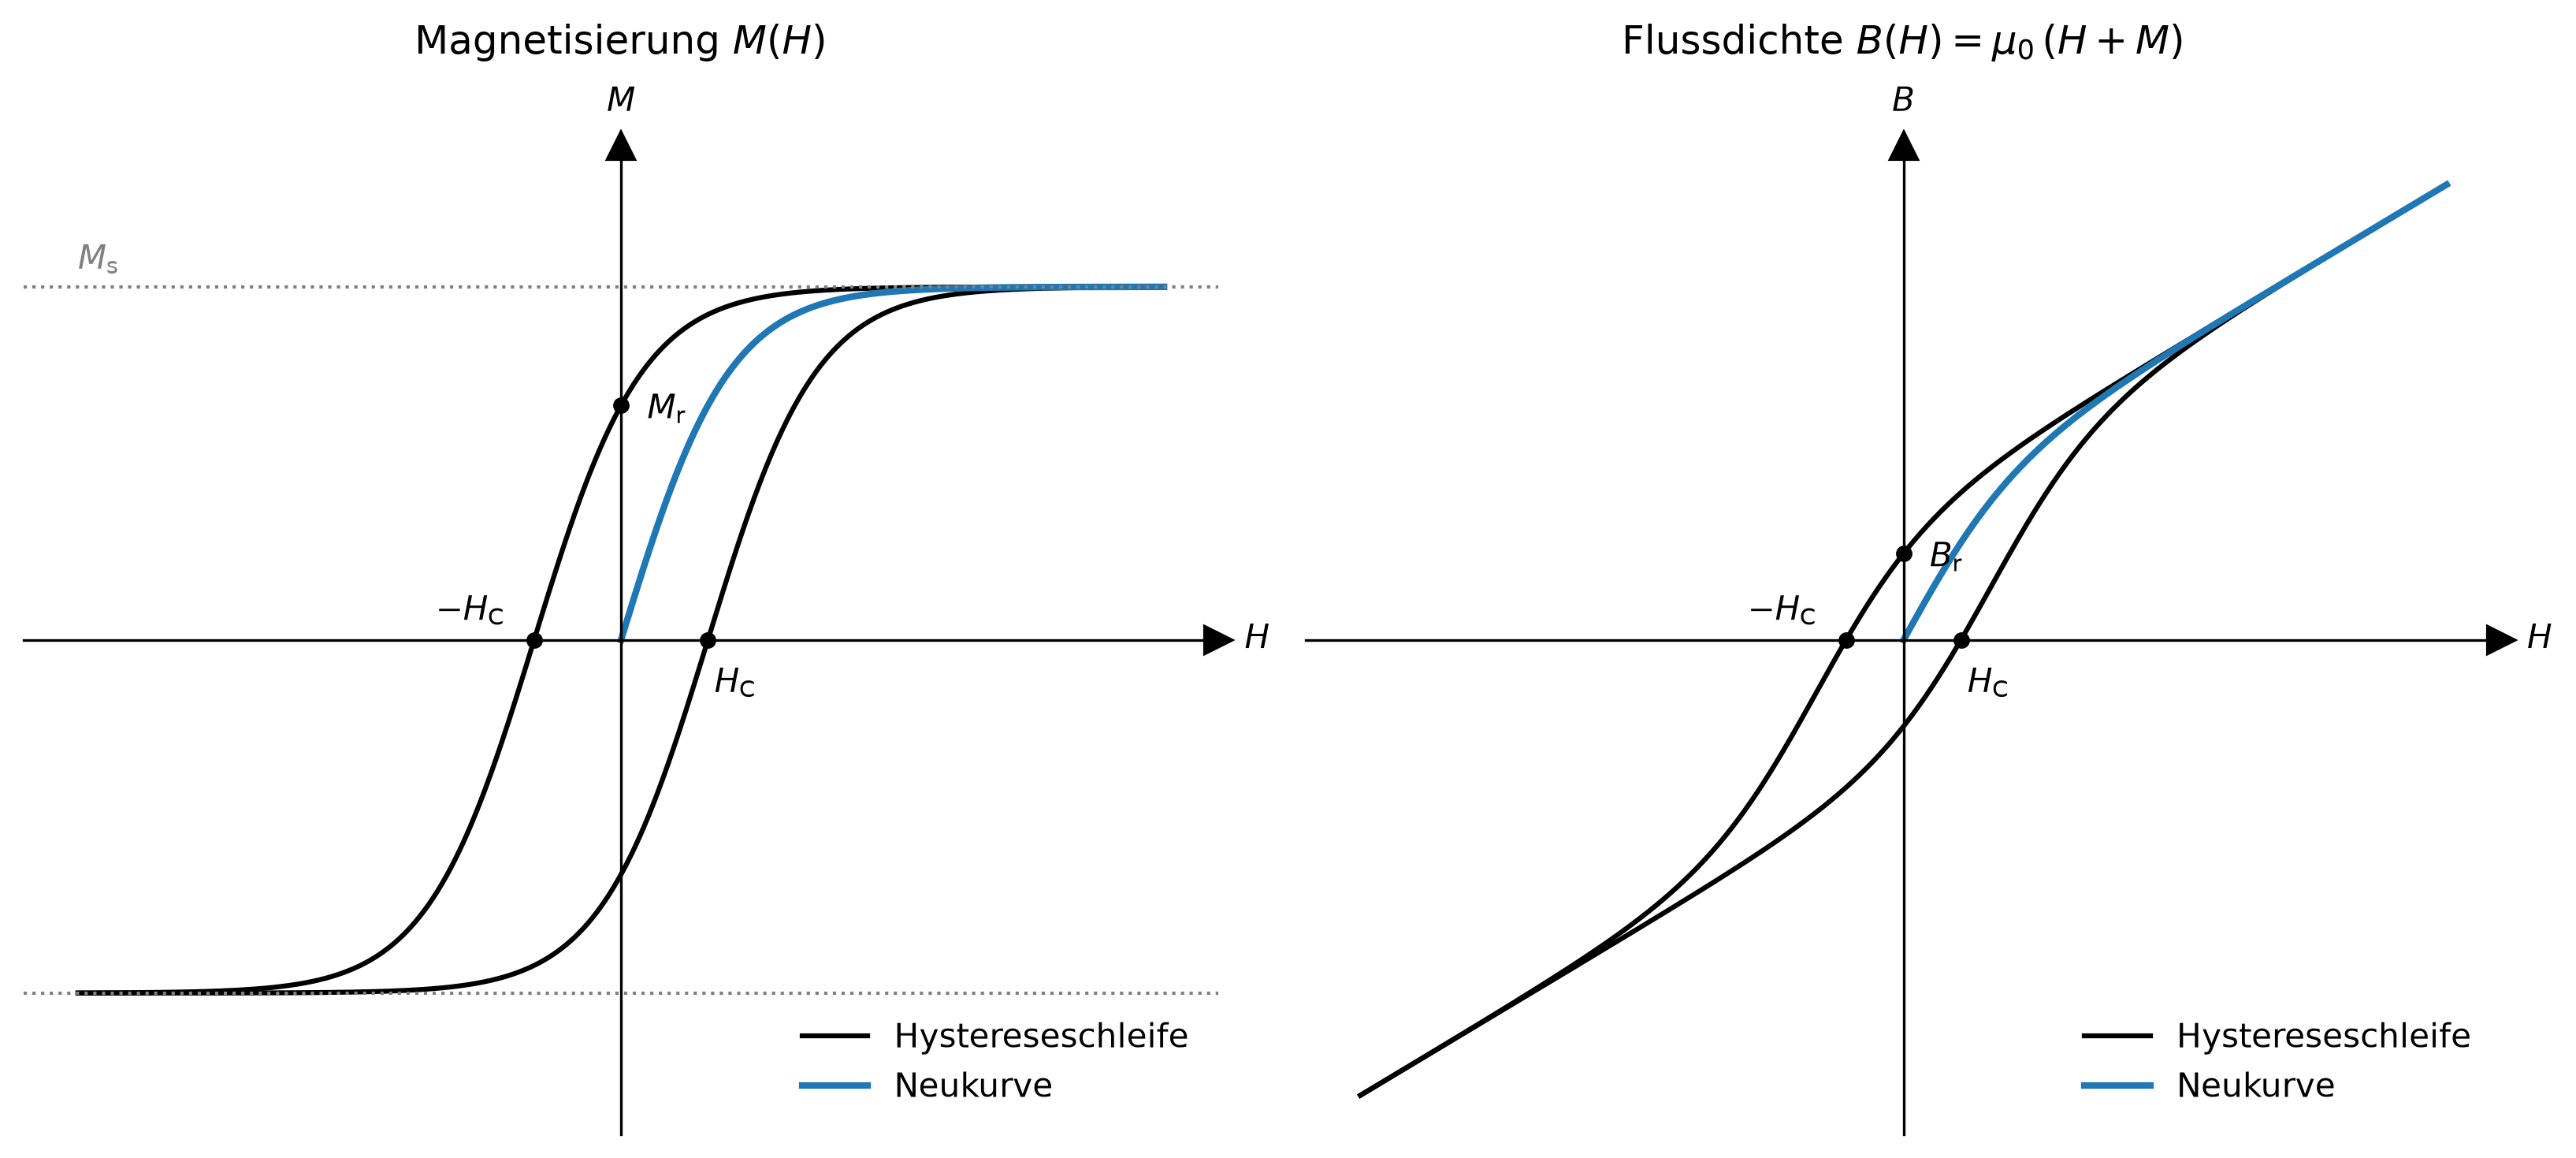
\includegraphics[width=\textwidth]{hysterese_skizze.png}
  \caption{Qualitativer Verlauf von $M(H)$ (links) und $B(H)$ (rechts) eines
           ferromagnetischen Stoffs mit Neukurve (blau) und Hystereseschleife
           (schwarz). Eigene Darstellung (Modellkurven, willkürliche Einheiten).}
  \label{fig:BH_MH}
\end{figure}

Abb.~\ref{fig:BH_MH} zeigt den qualitativen Verlauf. Es gilt $B=\mu_0(H+M)$ (fm.3).
$M(H)$ sättigt bei $M_\mathrm{s}$, $B(H)$ steigt auch danach mit der Steigung
$\mu_0$ weiter an. Beide Kurven zeigen Hysterese und Remanenz
($B_\mathrm{r}=\mu_0M_\mathrm{r}$). Die Neukurve (blau) beschreibt die erstmalige
Magnetisierung aus dem entmagnetisierten Zustand und liegt innerhalb der
Schleife. Die Koerzitivfeldstärke der $B(H)$-Kurve ($B=0$) ist betragsmäßig
kleiner als die der $M(H)$-Kurve ($M=0$).

\subsection{Entmagnetisieren eines ferromagnetischen Körpers}
\begin{itemize}
  \item Wechselfeld mit langsam auf null abnehmender Amplitude
  \item Erhitzen über die Curie-Temperatur ($T_\mathrm{C}^{\text{Fe}}\approx\SI{740}{\celsius}$) und Abkühlen ohne äußeres Feld
  \item mechanische Erschütterung (nur teilweise Entmagnetisierung)
\end{itemize}

\subsection{Querspalt, Längsspalt, transversale und longitudinale Hallsonde}
\label{sec:spalte}
\begin{itemize}
  \item \textbf{Querspalt} (senkrecht zu $\vec B$): Wegen $\nabla\cdot\vec B=0$
        (fm.1) ist $B$ stetig, also $B_\mathrm{E}=B_\mathrm{L}$ (fm.11). Mit der
        \emph{transversalen} Sonde (empfindlich senkrecht zur Sondenfläche)
        misst man direkt $B$ im Eisen.
  \item \textbf{Längsspalt} (parallel zu $\vec B$): Wegen
        $\nabla\times\vec H=\vec j=0$ (fm.2, fm.12) ist $H$ stetig, also
        $H_\mathrm{E}=H_\mathrm{L}$ (fm.14) $=B_\mathrm{L}/\mu_0$ (fm.15). Die
        \emph{longitudinale} Sonde (empfindlich in Richtung der Sondenachse)
        misst $B_\mathrm{L}$ und liefert daraus $H$ im Eisen.
\end{itemize}

\subsection{Warum müssen die Spalte eng sein?}
Enge Spalte stören die Magnetisierungsverteilung kaum, verringern Streu- und
entmagnetisierende Felder und halten den zusätzlichen magnetischen Widerstand
klein. Nur so gelten die Näherungen $B_\mathrm{E}=B_\mathrm{L}$ (fm.11) bzw.\
$H_\mathrm{E}=H_\mathrm{L}$ (fm.14).

\subsection{$\vec B$ bei nicht-durchgehendem Querspalt}
Nein, im Allgemeinen nicht. Ein Teil des Flusses kann über die verbleibenden
Eisenbrücken ausweichen, und es entstehen Streufelder. Die Flussdichte im Spalt
ist dann meist kleiner als bei einem durchgehenden Spalt.

\subsection{Wirkungsweise einer Hallsonde}
\label{sec:hall}
Durch ein Halbleiterplättchen fließt ein Strom $I$. Steht $\vec B$ senkrecht zur
Stromrichtung, lenkt die Lorentzkraft die Ladungsträger seitlich ab, und es
entsteht quer eine Hallspannung $U_\mathrm{H}\propto I\,B$. Gemessen wird also
die Flussdichte-Komponente senkrecht zu Strom und Hallspannung. Geometriebedingte
Nullfeldsignale (Offset) lassen sich eliminieren, indem man bei umgekehrtem Feld
(bzw.\ um \SI{180}{\degree} gedrehter Sonde) misst und mittelt, oder indem man
die Sonde bei $B=0$ abgleicht.

\subsection{Feld an den Enden einer langen Spule}
\label{sec:spulenende}
Am Spulenende liegen nur auf einer Seite Windungen, im Mittelpunkt auf beiden
Seiten. Das Feld am Ende beträgt daher etwa die Hälfte des Feldes im
Mittelpunkt.

\subsection{Feldstärke auf der Symmetrieachse einer Spule}
\label{sec:Hz}
Für eine Zylinderspule mit Gesamtwindungszahl $n$, Länge $l$, Radius $R$ und
Strom $I$ gilt auf der Symmetrieachse
\begin{equation}
  H(z)=\frac{nI}{2l}\left[
  \frac{z+\frac l2}{\sqrt{R^2+\left(z+\frac l2\right)^2}}
  -\frac{z-\frac l2}{\sqrt{R^2+\left(z-\frac l2\right)^2}}\right]
  \label{eq:Hz}
\end{equation}
Für $z=0$ folgt $B(0)=\mu_0H(0)=\mu_0\,nI/\sqrt{l^2+4R^2}$.
Parameter: $n=500$, $I=\SI{2.5}{\ampere}$, $R=D/2=\SI{2.75}{\centi\meter}$.
Die Vorbereitungsaufgabe nennt $l=\SI{8}{\centi\meter}$, die Spule im Versuch hat
$l=\SI{7.2}{\centi\meter}$. Beide Fälle sind dargestellt.

\begin{figure}[H]
  \centering
  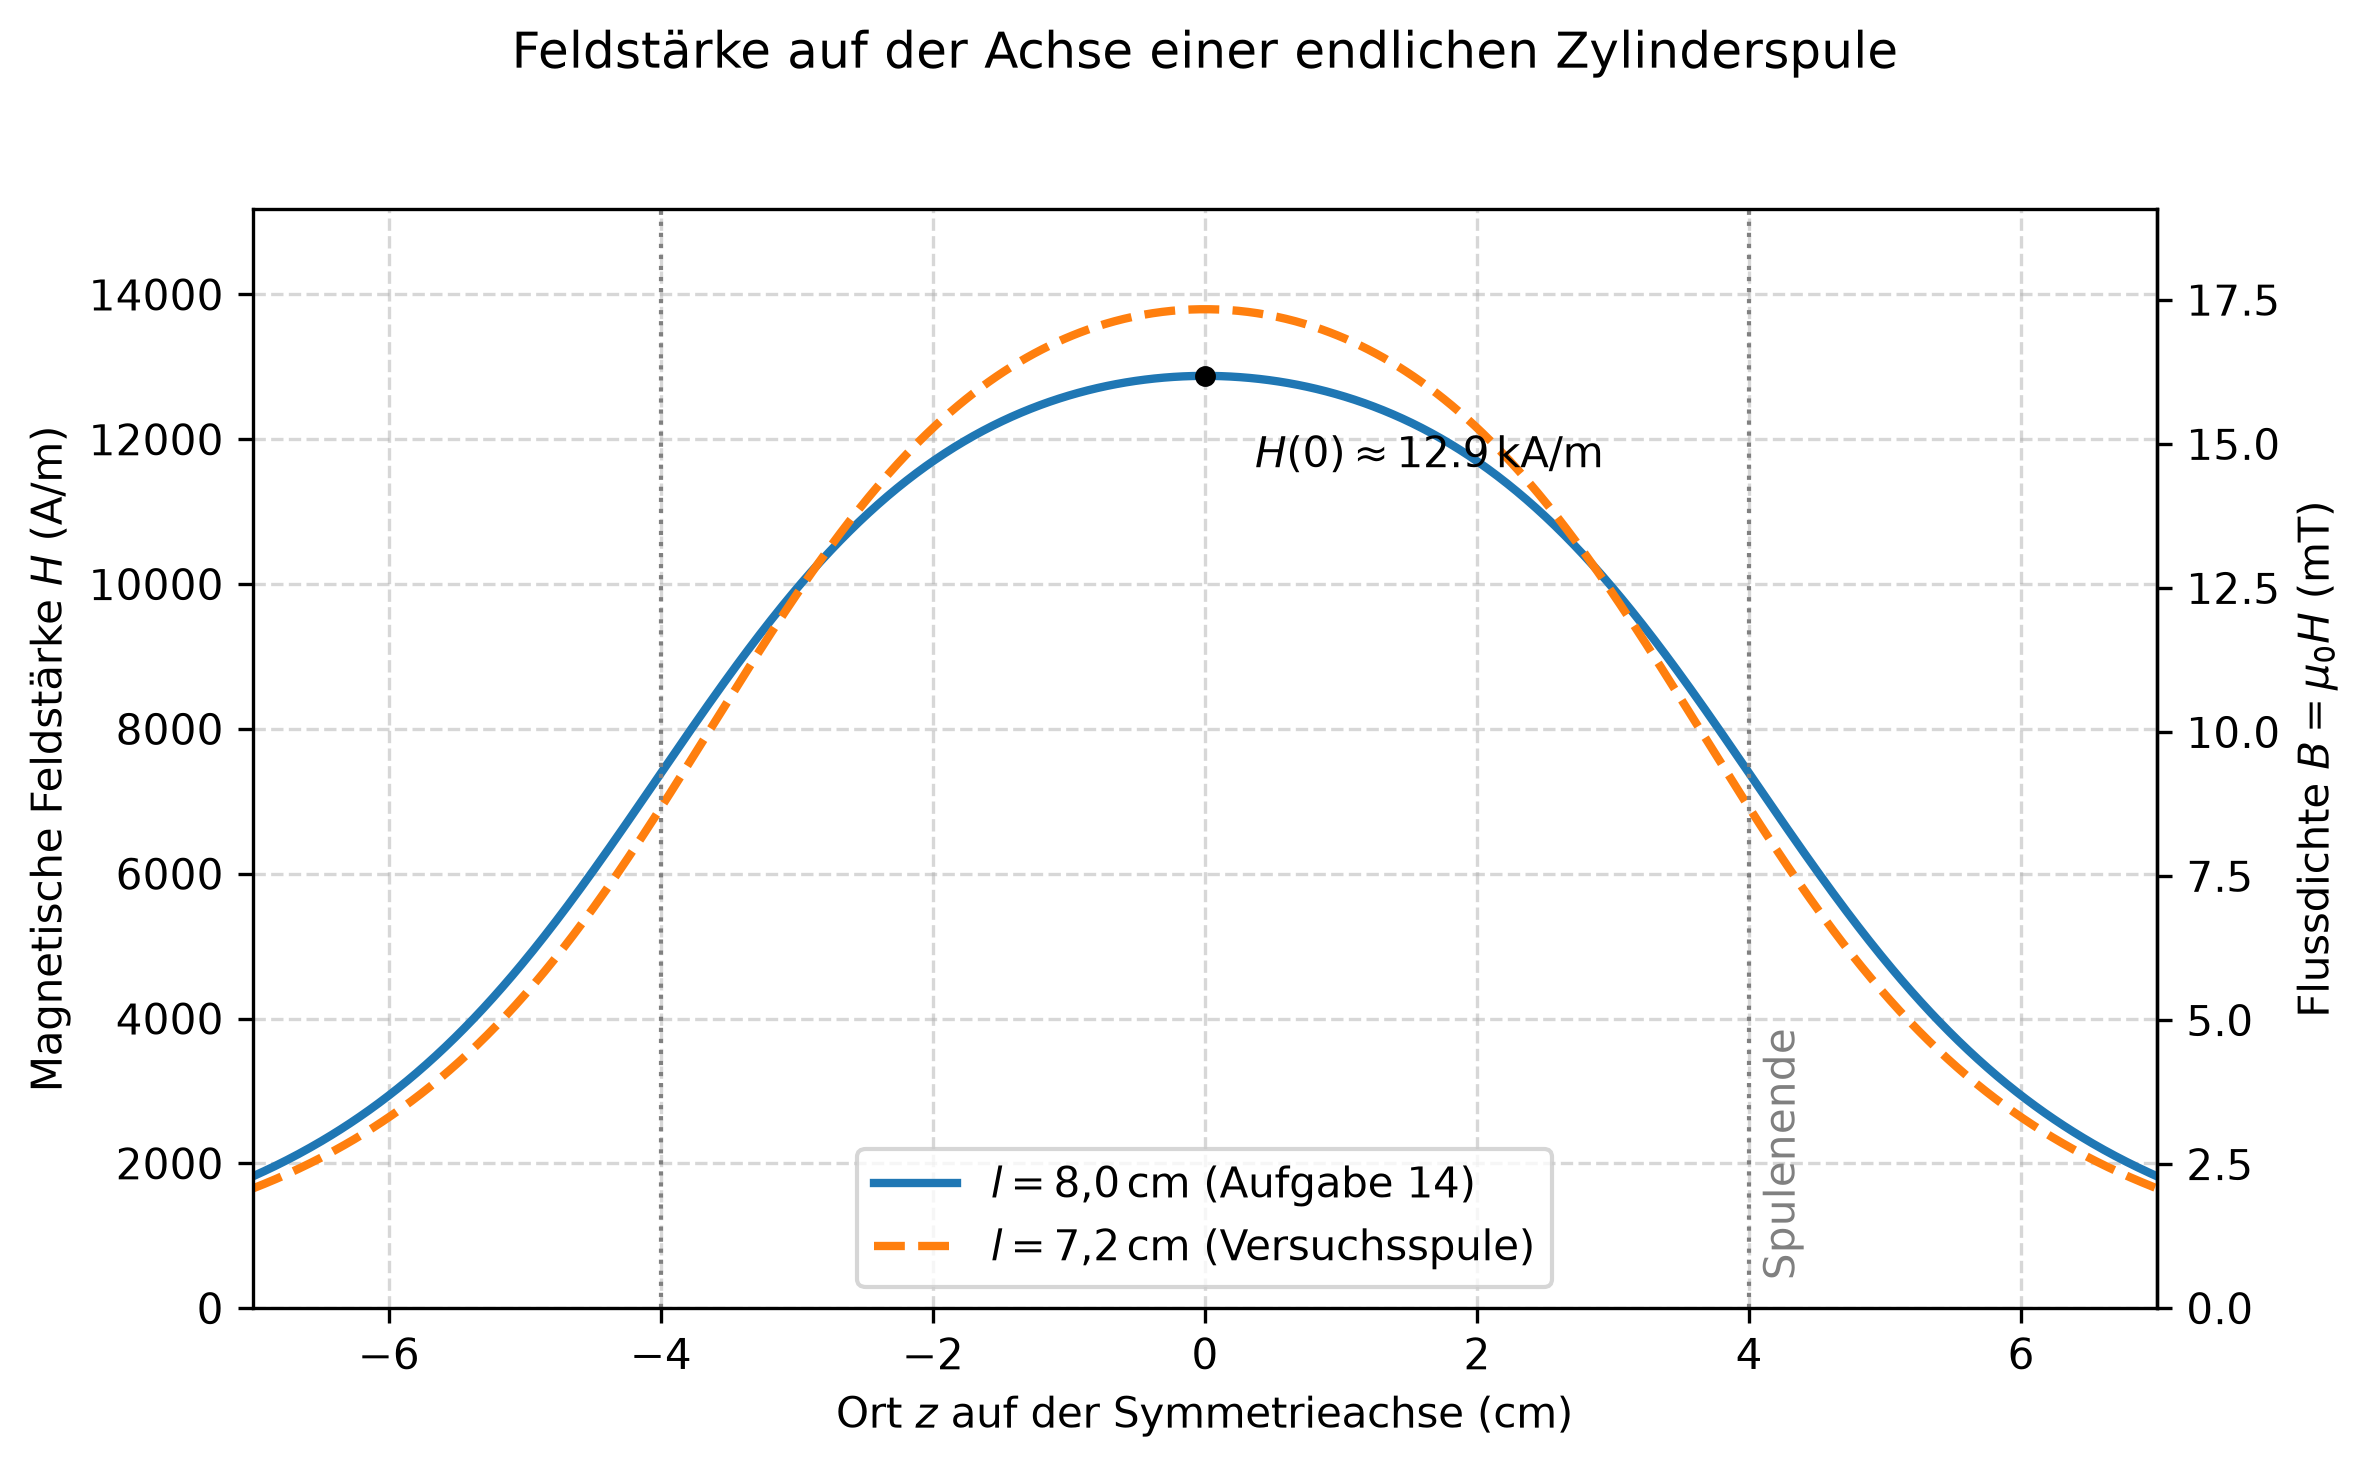
\includegraphics[width=0.85\textwidth]{hz_spule.png}
  \caption{Magnetische Feldstärke $H(z)$ auf der Symmetrieachse einer
           Zylinderspule nach Gl.~\eqref{eq:Hz} für $n=500$,
           $I=\SI{2.5}{\ampere}$, $D=\SI{5.5}{\centi\meter}$ und
           $l=\SI{8}{\centi\meter}$ (durchgezogen) bzw.\
           $l=\SI{7.2}{\centi\meter}$ (gestrichelt). Die rechte Achse zeigt
           $B=\mu_0H$. Eigene Darstellung.}
  \label{fig:Hz_theorie}
\end{figure}

Die Feldstärke ist in der Spulenmitte maximal und fällt zu den Enden hin ab.
Für $l=\SI{8}{\centi\meter}$ ergibt sich $H(0)\approx\SI{12.9}{\kilo\ampere\per\meter}$,
also $B(0)\approx\SI{16.2}{\milli\tesla}$, für $l=\SI{7.2}{\centi\meter}$
$B(0)\approx\SI{17.3}{\milli\tesla}$. An den Spulenenden beträgt die Feldstärke
etwa \SIrange{57}{59}{\percent} des Maximalwerts. Das liegt über der Abschätzung
„etwa die Hälfte“ aus Abschnitt~\ref{sec:spulenende}, weil die Spule kurz ist und
ihr Radius nicht klein gegen die Länge ist.

\subsection{Betrag des Erdmagnetfelds}
$B_\mathrm{Erde}\approx\SIrange{25}{65}{\micro\tesla}=\SIrange{0.25}{0.65}{\gauss}$
(mit $\SI{1}{\tesla}=\SI{10000}{\gauss}$). In Deutschland beträgt es ca.\ \SI{48}{\micro\tesla}.

\subsection{Anwendungen ferromagnetischer Stoffe}
Transformatoren, Motoren und Generatoren (Flussführung), Relais und Schütze,
magnetische Datenspeicher, Lautsprecher und Dauermagnete, magnetische
Abschirmungen.

\clearpage

% ======================= Geräte =======================
\section{Geräte und Aufbau}
\begin{itemize}
  \item Feldmessgerät (PHYWE) mit longitudinaler Hallsonde
  \item Feldmessgerät (PHYWE) mit transversaler Hallsonde
  \item Luftspule ($n=500$, $l=\SI{7.2}{\centi\meter}$, $D=\SI{5.5}{\centi\meter}$)
  \item gerader Eisenkern mit Längsbohrung, an einem Ende zäpfchenförmig verjüngt
  \item Kern mit Querspalt und Bohrung (Experimentiertrafo) für die Hysterese-Messung
  \item Netzgerät als Stromquelle (Strom bis etwa \SI{3.5}{\ampere})
  \item Kompass
  \item Multimeter, Stativmaterial
\end{itemize}

\clearpage

% ======================= 3 Durchführung =======================
\section{Durchführung und Auswertung}

% ---------- 3.1 ----------
\subsection{Test der Hallsonden mit Hilfe des Erdmagnetfelds}
\label{sec:erde}
Die Richtung des Erdmagnetfelds wurde mit einer Kompassnadel bestimmt, wobei
sich keine Eisenteile in der Nähe befanden, damit die Nadel nur dem
Erdfeld folgt. Die ermittelte Richtung wurde nicht notiert.

Anschließend wurde die Hallsonde in verschiedenen Orientierungen zum Erdfeld
gehalten (senkrecht, parallel und antiparallel, wie in der Anleitung
vorgesehen), und der Nullpunkt wurde am Nullregler des Messgeräts abgeglichen.
Der Regler wurde so lange verstellt, bis die Anzeige möglichst konstant bei null
lag. Damit ist der Offset der Sonde (Nullfeldsignal, vgl.\
Abschnitt~\ref{sec:hall}) kompensiert. Dies geschah sowohl für die longitudinale
als auch die transversale Sonde.

Der Abgleich betrifft nur den Nullpunkt. Das Erdfeld (ca.\ \SI{48}{\micro\tesla})
ist um mehr als zwei Größenordnungen schwächer als die Felder der späteren
Messungen (bis etwa \SI{30}{\milli\tesla} in den Spulenmessungen, über
\SI{1}{\tesla} in der Hysterese). Beobachtungen zur Abhängigkeit der Anzeige von
der Orientierung wurden nicht festgehalten. Ob die Sonde das Erdfeld
erwartungsgemäß abbildet, lässt sich daher nicht beurteilen, und eine Aussage
über die Empfindlichkeit der Sonde ist aus diesem Test nicht möglich. Für die
Messunsicherheit werden die in Abschnitt~\ref{sec:unsicher} genannten
Abschätzungen verwendet.

% ---------- 3.2 ----------
\subsection{Magnetfeld einer Luftspule}
\label{sec:luft}
Die Luftspule ($l=\SI{7.2}{\centi\meter}$, $D=\SI{5.5}{\centi\meter}$, $n=500$)
wurde mit $I=\SI{2.5}{\ampere}$ betrieben. Die longitudinale Hallsonde wurde
entlang der Symmetrieachse verschoben und die Flussdichte in Schritten von
\SI{0.5}{\centi\meter} aufgenommen (zwischen $-10$ und $-\SI{7}{\centi\meter}$
teils \SI{1}{\centi\meter}), im Bereich von etwa $-10{,}5$ bis
$+\SI{10.5}{\centi\meter}$. Als Nullpunkt des Abstands sollte die Mitte der
Spulenwicklung dienen. Die Sondenposition wurde in den Abstand vom
Spulenmittelpunkt umgerechnet, indem der Abstand der Sonde vom Rand der Spule
gemessen wurde.

\begin{figure}[H]
  \centering
  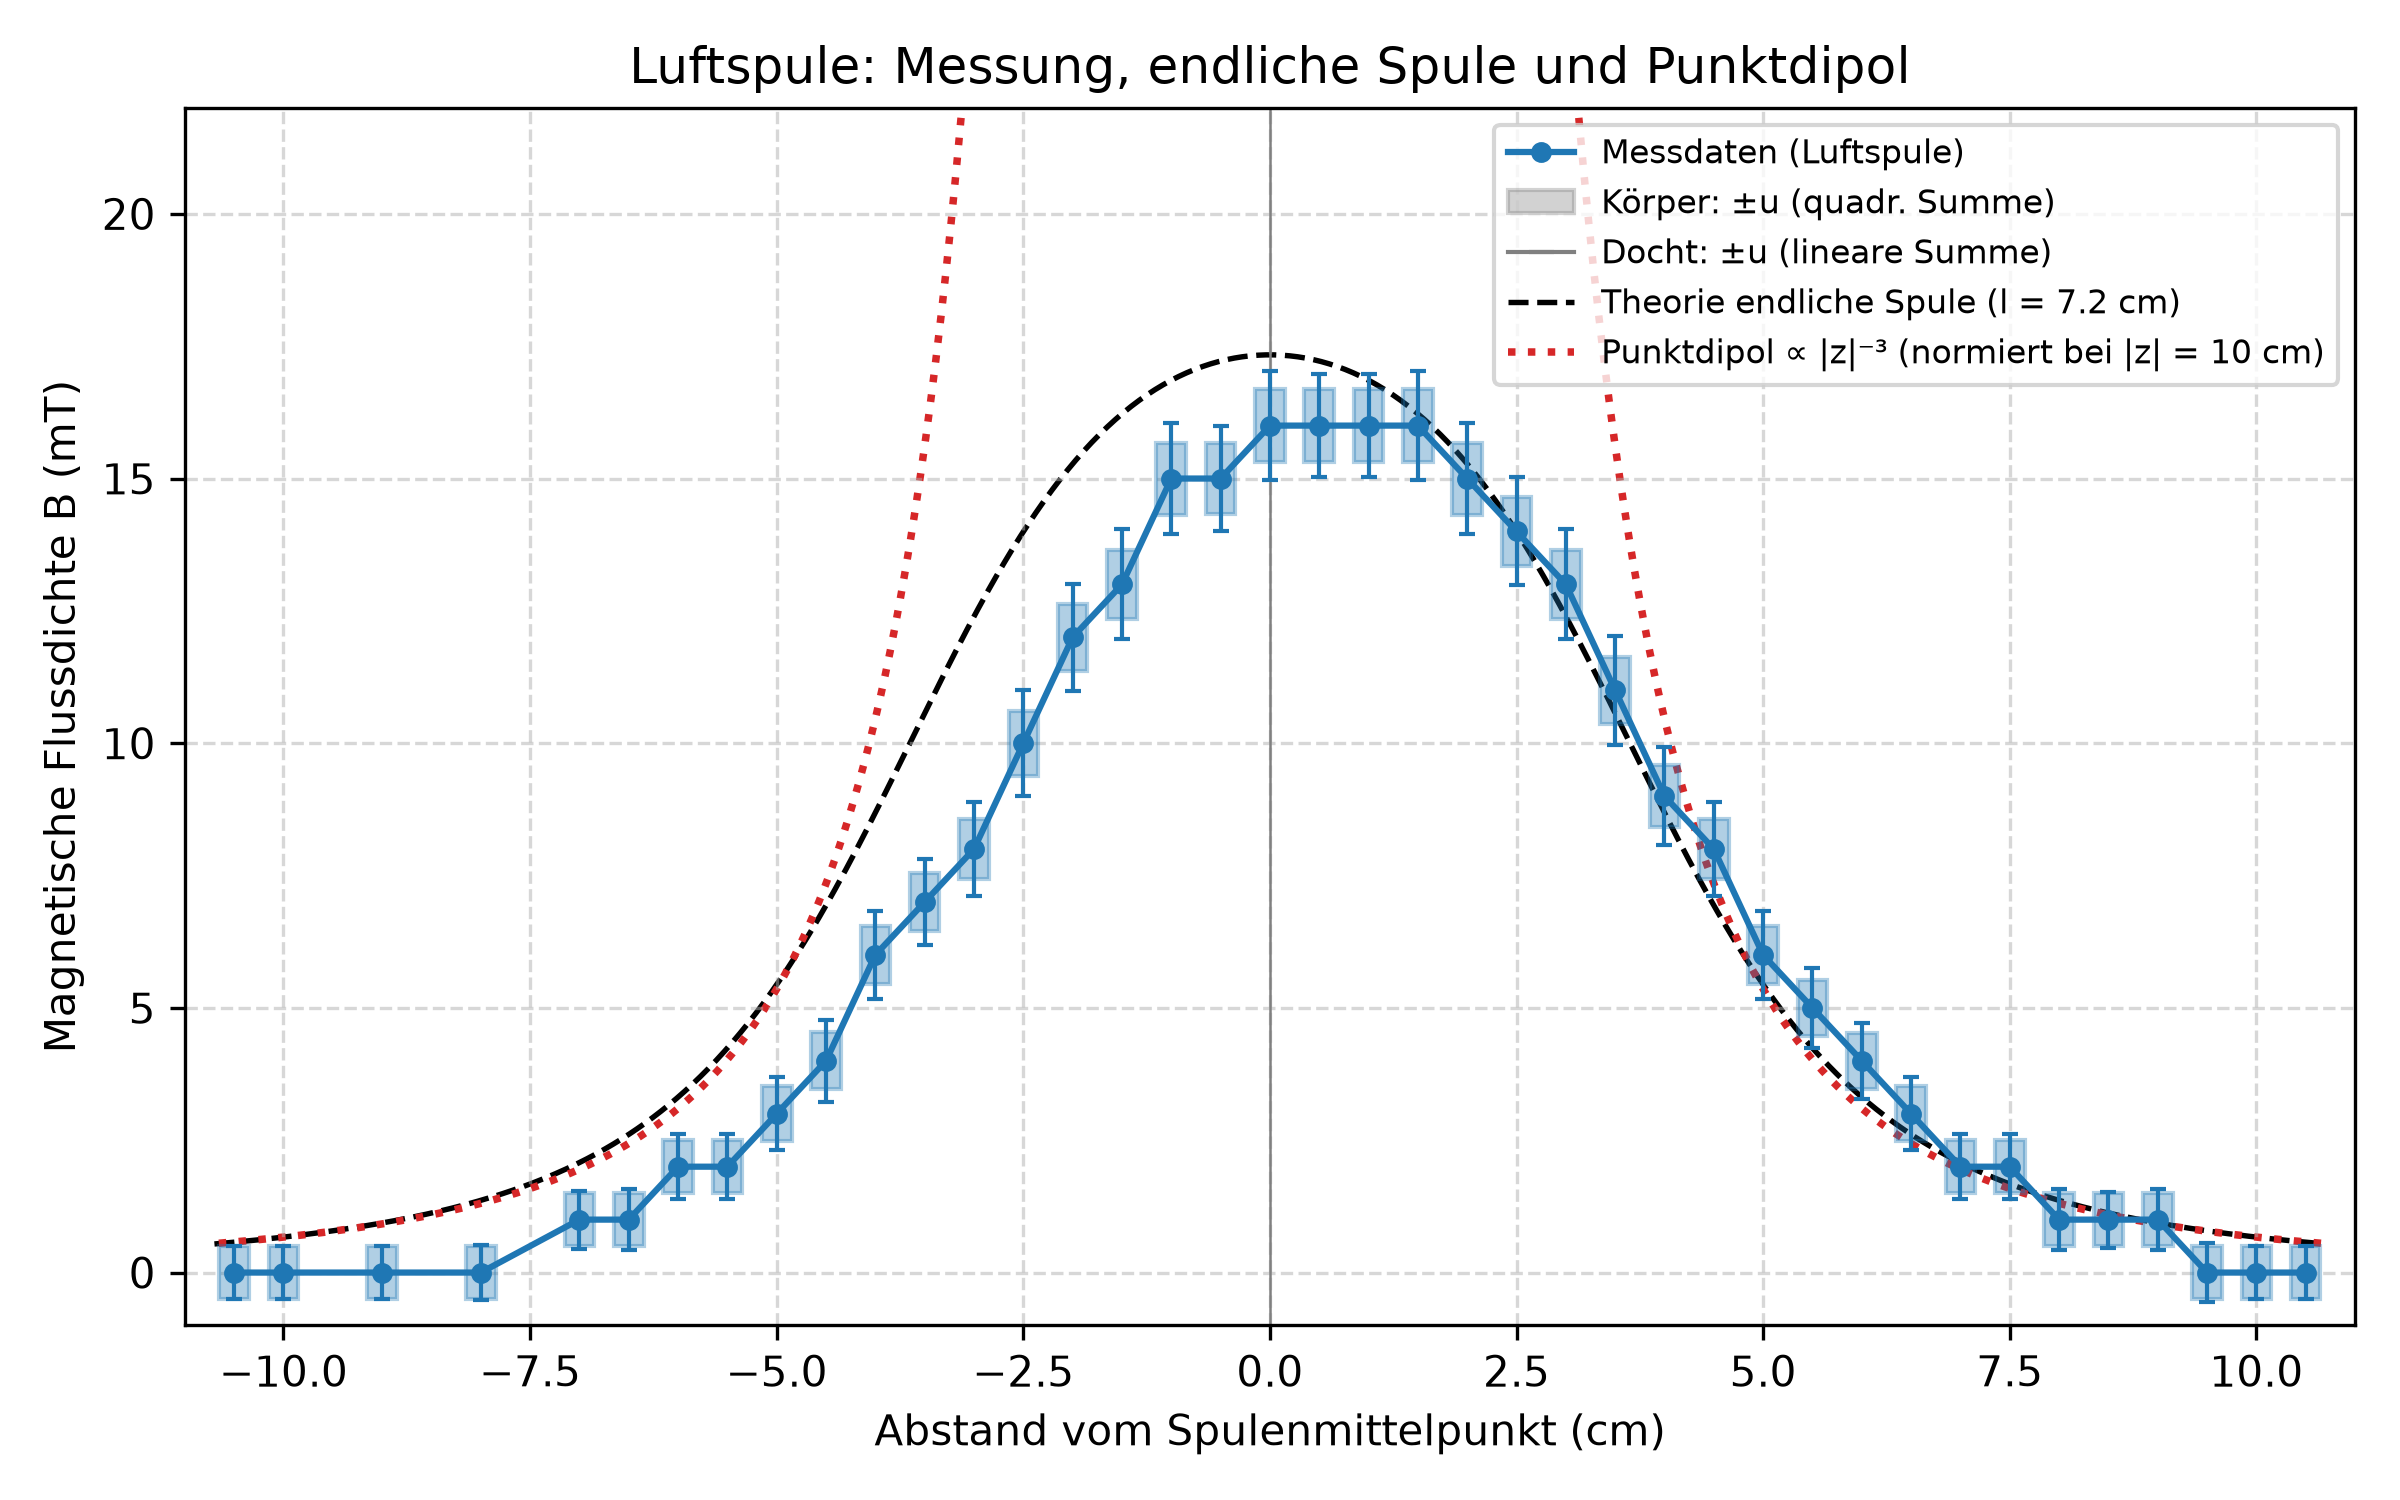
\includegraphics[width=0.85\textwidth]{vergleich_luftspule.png}
  \caption{Magnetische Flussdichte $B$ der Luftspule entlang der Symmetrieachse
    ($I=\SI{2.5}{\ampere}$), Messdaten unkorrigiert. Kerzen: Körper $=\pm u_B$
    (quadratische Summe aus \SI{3}{\percent} Geräteunsicherheit,
    $\pm\SI{0.5}{\milli\tesla}$ Ablesung und Positionsfehler
    $\pm\SI{0.05}{\centi\meter}$, über die Steigung umgerechnet), Docht $=$ lineare
    Summe (Worst Case). Die Breite der Körper dient nur der Darstellung.
    Gestrichelt: Theoriekurve für eine endliche Zylinderspule nach
    Gl.~\eqref{eq:Hz} mit $n=500$, $I=\SI{2.5}{\ampere}$,
    $R=\SI{2.75}{\centi\meter}$, $l=\SI{7.2}{\centi\meter}$ und $B=\mu_0H$, auf
    $z=0$ zentriert und nicht an die Daten angepasst. Rot gepunktet: Punktdipol-Näherung $B\propto|z|^{-3}$, bei $|z|=\SI{10}{\centi\meter}$ auf die Theoriekurve der endlichen Spule normiert (nicht an die Daten angepasst) und nur für $|z|\ge\SI{3}{\centi\meter}$ gezeichnet.}
  \label{fig:luftspule}
\end{figure}

\textbf{Beschreibung:} Das Feld ist glockenförmig mit einem Plateau von etwa
\SI{16}{\milli\tesla} zwischen \SI{0}{\centi\meter} und \SI{1.5}{\centi\meter}.
Zu beiden Seiten fällt es auf nahezu null ab (Anzeige $0$ ab etwa
$-\SI{8}{\centi\meter}$ bzw.\ $+\SI{9.5}{\centi\meter}$). Am Maximum beträgt die
Unsicherheit $u_B\approx\SI{0.7}{\milli\tesla}$ (Körper) bzw.\
\SI{1.0}{\milli\tesla} (Docht).

\textbf{Vergleich mit der Theorie:} Für die Spulenmitte erwartet man
\begin{equation}
  B(0)=\frac{\mu_0 nI}{\sqrt{l^2+4R^2}}\approx\SI{17.3}{\milli\tesla}
  \quad(l=\SI{7.2}{\centi\meter}).
\end{equation}
Die Wicklungslänge von \SI{7.2}{\centi\meter} ist korrekt, die Theoriekurve
verwendet daher die Nennwerte. Das gemessene Maximum liegt um
$-\SI{1.3}{\milli\tesla}$ ($\approx-\SI{7.5}{\percent}$) unter dem theoretischen
Wert. Berücksichtigt man zusätzlich die \SI{3}{\percent} Stromunsicherheit auf
der Theorieseite ($\pm\SI{0.5}{\milli\tesla}$), beträgt die kombinierte
Unsicherheit quadratisch etwa \SI{0.9}{\milli\tesla} und als Worst Case
\SI{1.5}{\milli\tesla}. Die Abweichung ist damit etwa das 1,5-Fache der
quadratischen Unsicherheit, liegt aber noch innerhalb der Worst-Case-Summe, sie
ist also nur schwach signifikant. Als Ursache kommt vor allem die geringe
Messerfahrung in Frage, da der Versuch der erste im Labor war: Die Sonde war
möglicherweise nicht exakt auf der Achse geführt oder leicht verkippt, und
Position und Anzeige wurden vermutlich nur grob bestimmt. Diese Beiträge sind in
$u_B$ nur teilweise erfasst, die tatsächliche Unsicherheit dürfte daher etwas
größer sein als eingezeichnet.

\textbf{Asymmetrie:} Die Halbwertspunkte ($B=\SI{8}{\milli\tesla}$) liegen bei
etwa $-\SI{3.0}{\centi\meter}$ und $+\SI{4.5}{\centi\meter}$. Die Kurve ist also
um etwa \SI{0.75}{\centi\meter} nach rechts verschoben. Die Halbwertsbreite
beträgt \SI{7.5}{\centi\meter} (Theorie: ca.\ \SI{8.0}{\centi\meter}) und stimmt
im Rahmen der Schrittweite von \SI{0.5}{\centi\meter} annähernd überein. Passend
zur Verschiebung liegt die Messung auf der negativen Seite unter und auf der
positiven Seite über der Theoriekurve (bei $-\SI{4}{\centi\meter}$:
\SI{6}{\milli\tesla} gegenüber \SI{8.7}{\milli\tesla}, bei
$+\SI{4}{\centi\meter}$: \SI{9}{\milli\tesla} gegenüber \SI{8.7}{\milli\tesla}).
Die Verschiebung ist rund 15-mal größer als die angesetzte
Positionsunsicherheit von \SI{0.05}{\centi\meter} und damit ein systematischer
Fehler. Am wahrscheinlichsten wurde die Spulenmitte falsch bestimmt, oder beim
Umrechnen der Sondenposition in den Abstand vom Spulenmittelpunkt ist ein Fehler
unterlaufen. Das lässt sich nicht mehr nachvollziehen. Die Messpunkte selbst sind
davon nicht betroffen, nur ihre Zuordnung zur Koordinatenachse. Eine nachträgliche
Korrektur der Daten wurde nicht vorgenommen.

\textbf{Punktdipol:} Für Abstände groß gegen die Spulenabmessungen
($l=\SI{7.2}{\centi\meter}$, $D=\SI{5.5}{\centi\meter}$) kann die Spule als
Punktdipol mit $B\propto|z|^{-3}$ genähert werden. Die Dipolkurve in
Abb.~\ref{fig:luftspule} ist bei $|z|=\SI{10}{\centi\meter}$ auf die Theorie der
endlichen Spule normiert. In der Nähe der Spule weicht sie stark ab: Bei
$|z|=\SI{3}{\centi\meter}$ liegt sie etwa beim Doppelten der Theorie der
endlichen Spule, bei $\SI{4}{\centi\meter}$ etwa \SI{20}{\percent} darüber, und
sie divergiert für $z\to0$. Ab etwa $|z|=\SI{5}{\centi\meter}$ stimmen beide
Kurven auf wenige Prozent überein. In diesem Bereich liegen die Messwerte
jedoch nur noch bei \SIrange{0}{6}{\milli\tesla} und sind auf ganze
\si{\milli\tesla} gerundet ($\pm\SI{0.5}{\milli\tesla}$). Zusammen mit der
Verschiebung der Koordinatenachse lässt sich der $|z|^{-3}$-Verlauf daher nur
grob prüfen, eine quantitative Aussage ist nicht möglich. Im Nahfeld ist die
Formel der endlichen Spule der geeignete Vergleich.

% ---------- 3.3 ----------
\subsection{Magnetfeld einer Spule mit geradem Eisenkern}
\label{sec:eisen}
In die Spule wurde ein gerader Eisenkern mit Längsbohrung eingesetzt. Er ist an
einem Ende zäpfchenförmig verjüngt (Flusskonzentrator). Das gerade Ende schloss
bündig mit der Spule ab, das verjüngte Ende ragte auf der negativen
$x$-Seite aus der Spule heraus. Gemessen wurde wie in
Abschnitt~\ref{sec:luft} bei $I=\SI{2.5}{\ampere}$ mit der longitudinalen Sonde,
die in der Bohrung des Kerns geführt wurde, in Schritten von
\SI{0.5}{\centi\meter} an den Flanken und \SI{1}{\centi\meter} im feldfreien
Bereich ($\pm\SI{7}{\centi\meter}$). Da das Koordinatensystem aus
Abschnitt~\ref{sec:luft} übernommen wurde, wirkt sich die dort vermutete
Verschiebung der Nullposition auch hier aus.

\begin{figure}[H]
  \centering
  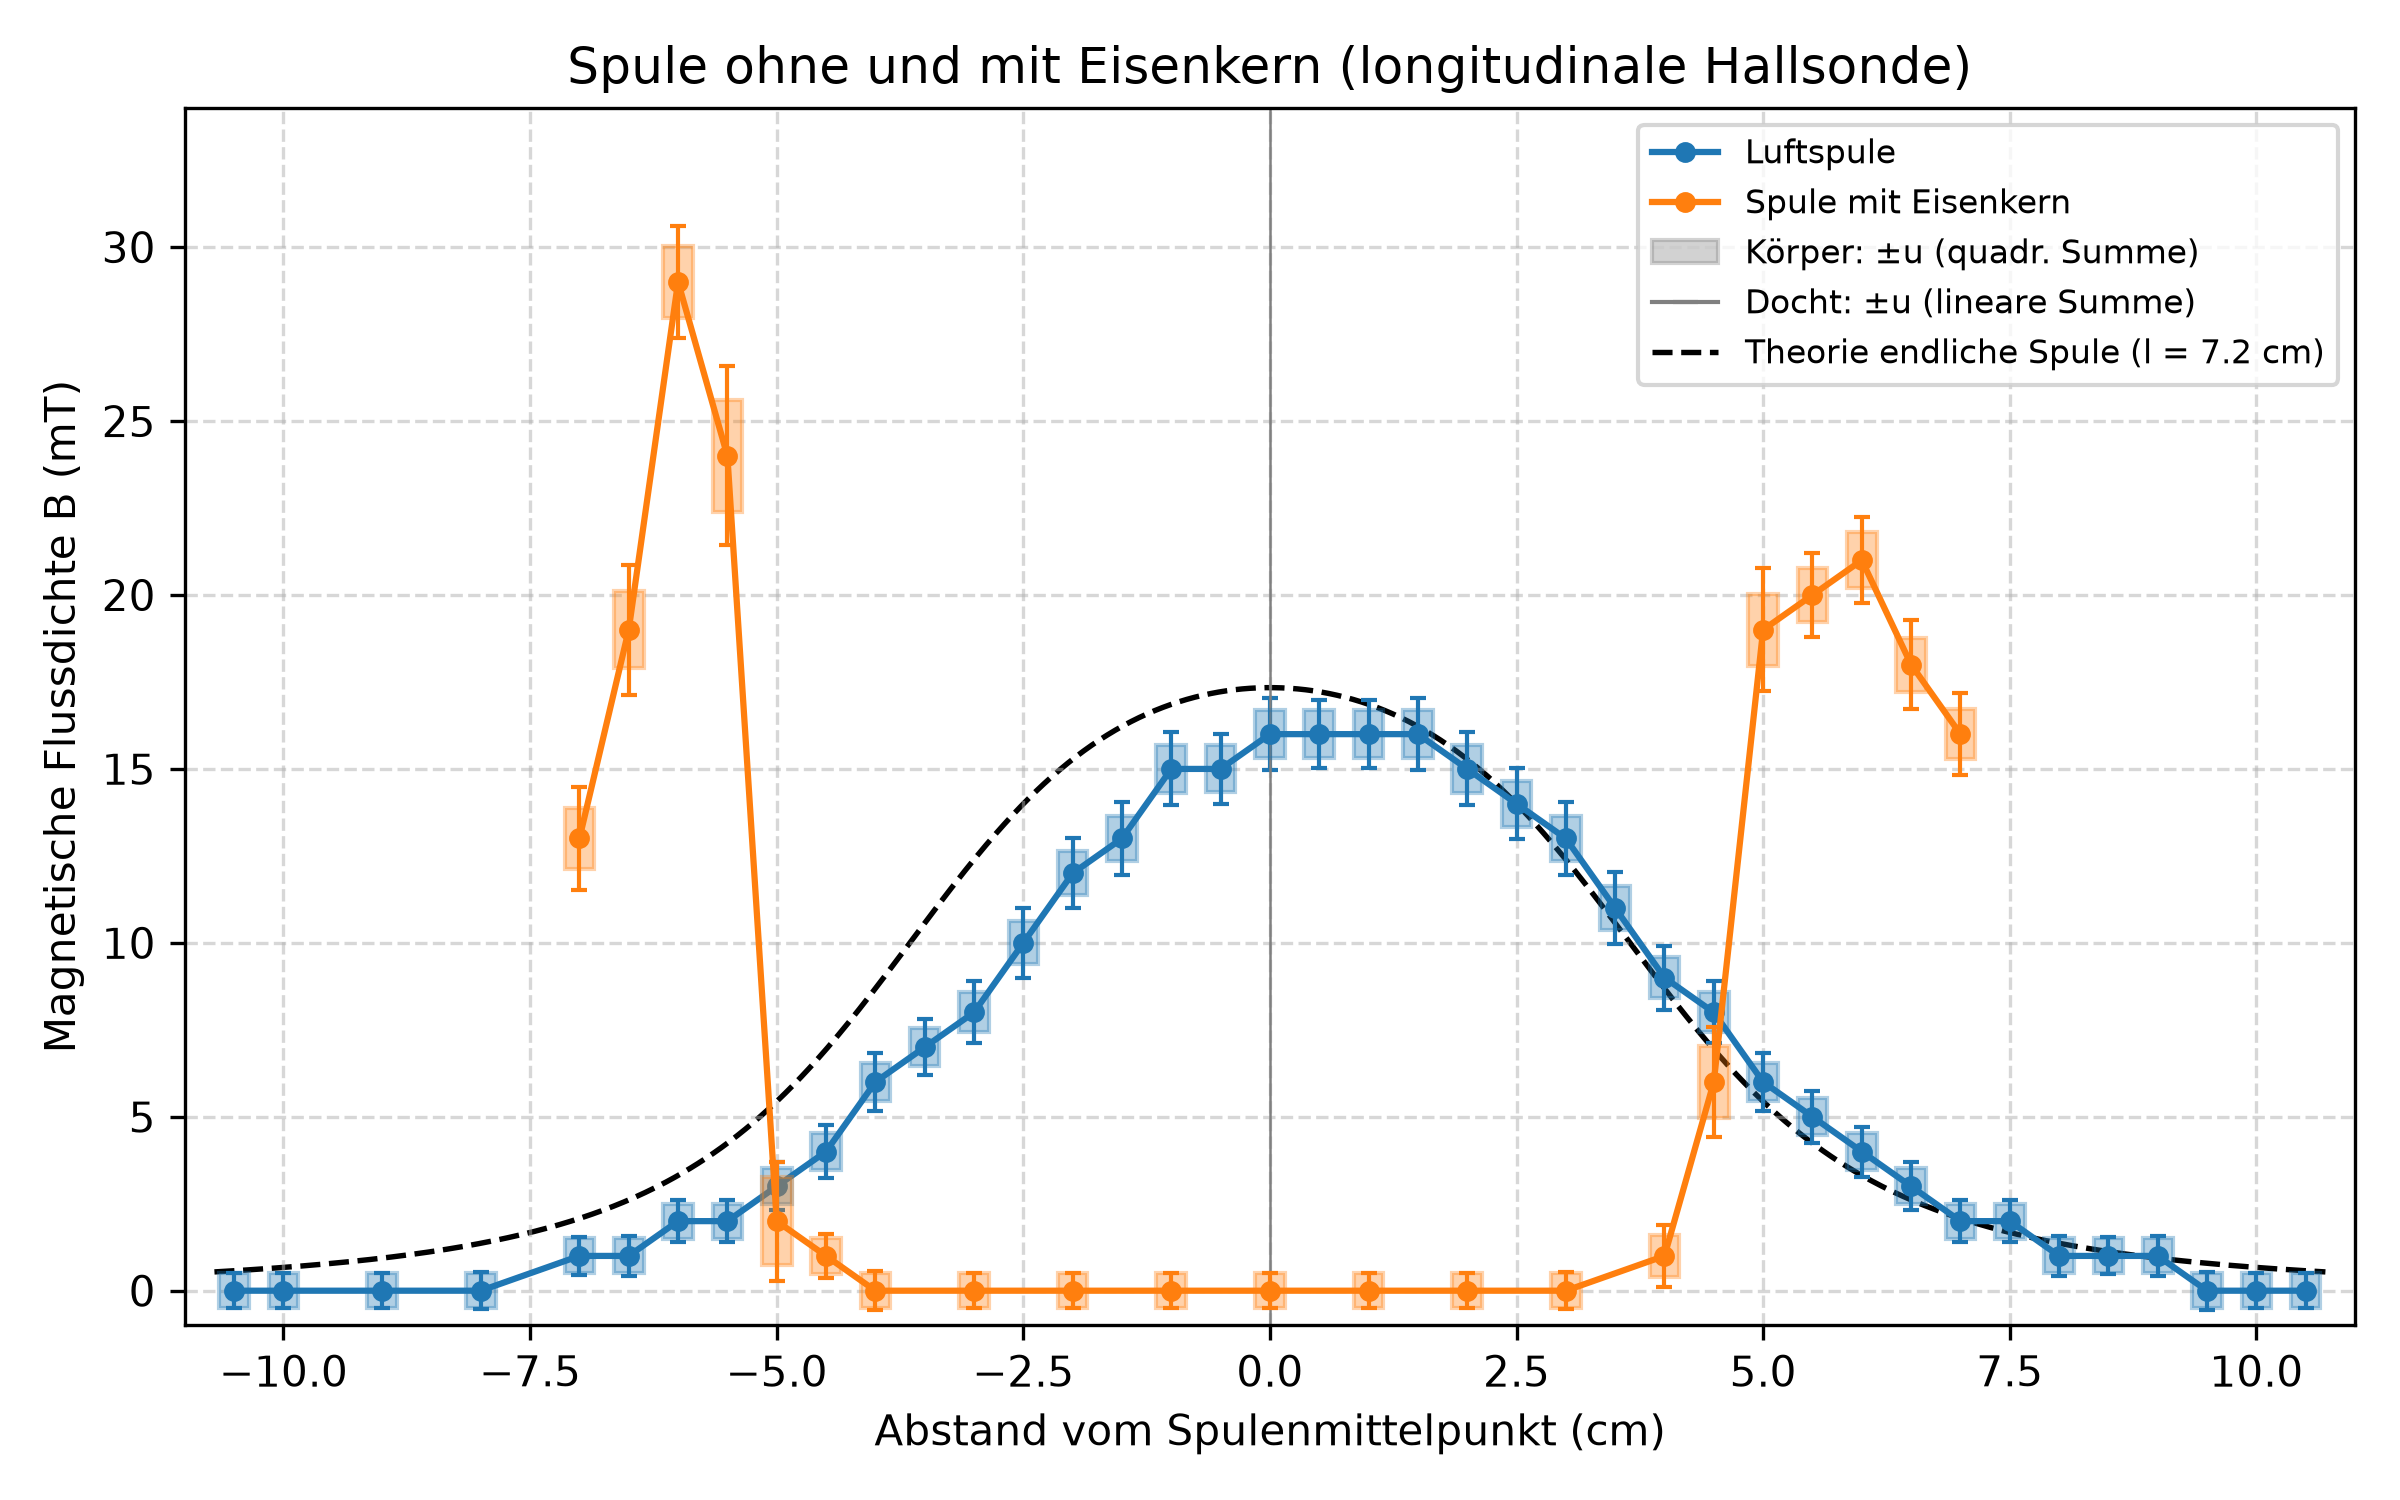
\includegraphics[width=0.85\textwidth]{vergleich_luft_eisen.png}
  \caption{Magnetische Flussdichte $B$ der Spule ohne (blau) und mit Eisenkern
         (orange) entlang der Symmetrieachse (longitudinale Hallsonde,
         $I=\SI{2.5}{\ampere}$), gleiche Achsen für beide Messungen, Messdaten
         unkorrigiert. Das verjüngte Ende des Kerns ragt auf der negativen Seite
         aus der Spule. Kerzen wie in Abb.~\ref{fig:luftspule}. Gestrichelt:
         Theorie der endlichen Spule ohne Kern.}
  \label{fig:eisenkern}
\end{figure}

\textbf{Beschreibung:} Im Bereich von etwa $-4$ bis $+\SI{3}{\centi\meter}$ ist die
gemessene Flussdichte praktisch null. Außerhalb davon steigt sie stark an und
erreicht zwei Maxima von etwa \SI{29}{\milli\tesla} (bei $-\SI{6}{\centi\meter}$)
und etwa \SI{21}{\milli\tesla} (bei $+\SI{6}{\centi\meter}$). Das höhere Maximum
liegt auf der Seite des verjüngten Endes (Flusskonzentrator). Die Länge des
Eisenkerns wurde nicht gemessen, die Lage der Kernenden lässt sich daher nur
grob aus dem Anstieg der Kurve abschätzen (etwa bei $-5$ bzw.\
$+\SI{4}{\centi\meter}$).

\textbf{Diskussion:}
\begin{itemize}
  \item \textbf{Feld in der Bohrung:} Im Bereich von etwa $-4$ bis
        $+\SI{3}{\centi\meter}$ lag die Anzeige der longitudinalen Sonde bei
        null. Dieses Ergebnis konnte im Rahmen des Versuchs nicht gedeutet
        werden. Es wurde nicht geprüft, ob die Sonde in der Bohrung richtig
        positioniert war oder ein Messfehler vorliegt. Eine quantitative
        Auswertung ist daher nicht möglich.
  \item \textbf{Maxima an den Kernenden:} Vermutlich verlässt die Sonde dort
        den Kern und misst das Streufeld, in dem der im Eisen geführte Fluss
        austritt. Da die Kernlänge nicht gemessen wurde, ist das nicht
        überprüfbar.
  \item \textbf{Plausibilität der Lage des flachen Kernendes:} Das flache Ende
        des Kerns schloss bündig mit der Spule ab, lag also bei
        $+l/2=+\SI{3.6}{\centi\meter}$. Mit der in Abschnitt~\ref{sec:luft}
        gefundenen Verschiebung der Koordinatenachse um etwa
        $+\SI{0.75}{\centi\meter}$ erscheint das Spulenende in den Messdaten
        bei etwa $+\SI{4.35}{\centi\meter}$ (gleiches Koordinatensystem
        vorausgesetzt). Der Anstieg der Kurve auf der positiven Seite beginnt
        zwischen $+4$ und $+\SI{4.5}{\centi\meter}$, also dort. Das stützt die
        Deutung der Verschiebung als Fehler bei der Bestimmung der
        Spulenmitte. Ein Beweis ist das nicht, da die Lage nur grob aus dem
        Anstieg der Kurve abgelesen ist. Auf der negativen Seite ist ein
        entsprechender Vergleich wegen der unbekannten Kernlänge nicht möglich.
  \item \textbf{Asymmetrie durch die Kernform:} Das verjüngte Ende wirkt als
        Flusskonzentrator. Der Fluss $\Phi=B\,A$ (fm.28) wird im Eisen geführt
        und tritt am verjüngten Ende durch eine kleinere Fläche aus, die
        Flussdichte steigt dort ($B\propto1/A$). Zusätzlich sind die Feldlinien
        an Spitzen dichter gebündelt (ähnlich dem Spitzeneffekt in der
        Elektrostatik). Am flachen Ende verteilt sich derselbe Fluss auf eine
        größere Fläche, das Maximum ist kleiner. Gemessen wurden etwa
        \SI{29}{\milli\tesla} am verjüngten Ende
        ($z\approx-\SI{6}{\centi\meter}$) und \SI{21}{\milli\tesla} am flachen
        Ende ($z\approx+\SI{6}{\centi\meter}$), das Verhältnis beträgt etwa
        $1{,}4\pm0{,}1$. Der Unterschied liegt deutlich über der
        Messunsicherheit und spiegelt die Geometrie des Kerns wider. Die Maxima
        sind nur durch wenige Punkte aufgelöst, und unmittelbar neben dem Maximum
        fällt die Kurve zwischen $-5{,}5$ und $\SI{-5}{\centi\meter}$ um bis zu etwa
        \SI{44}{\milli\tesla\per\centi\meter} ab. Ein Positionsfehler von
        $\SI{0.05}{\centi\meter}$ entspräche dort etwa $\SI{2}{\milli\tesla}$. Das
        wahre Maximum kann außerdem zwischen zwei Messpunkten liegen. Das ändert
        nichts am Gesamtbild. Da die Kernlänge nicht bestimmt wurde, kann die
        Lage der Maxima relativ zu den Kernenden nicht quantitativ diskutiert
        werden.
  \item \textbf{Relative Permeabilität:} Aus diesen Messungen lässt sich
        $\mu_\mathrm{r}$ nicht bestimmen. Die longitudinale Sonde liefert nur
        $H_\mathrm{E}$, und in der Bohrung wurde kein auswertbares Feld
        gemessen. $B_\mathrm{E}$ liegt nur für den Aufbau der
        Hysterese-Messung vor, dort jedoch ohne auswertbares $H_\mathrm{E}$.
\end{itemize}

% ---------- 3.4 ----------
\subsection{Ermittlung der Hysteresekurve eines Eisenkerns \glqq von Hand\grqq}
\label{sec:hyst}
Für diesen Teil wurde ein Kern mit Querspalt und Bohrung verwendet.
Die Flussdichte $B$ wurde mit der transversalen Hallsonde im Querspalt gemessen
(Abschnitt~\ref{sec:spalte}, $B_\mathrm{E}=B_\mathrm{L}$). Die longitudinale Sonde
wurde etwa bis zur Hälfte in die Bohrung eingeführt (Eindringtiefe nicht
nachgemessen), um Streufelder möglichst gering zu halten.

Der Spulenstrom wurde ausgehend von etwa $-\SI{3.5}{\ampere}$ in Schritten von
etwa \SIrange{0.1}{0.3}{\ampere} \emph{monoton} bis etwa $+\SI{3.3}{\ampere}$ und
anschließend wieder bis etwa $-\SI{3.4}{\ampere}$ verändert (Darstellung mit
umgekehrter Polung gegenüber der Anzeige, siehe unten). Bei einer Umkehr der
Stromrichtung mitten im Verlauf würde eine Nebenschleife entstehen, da der
Zustand von der Vorgeschichte abhängt. Ein kurzzeitiges Erhöhen auf bis zu
\SI{5}{\ampere}, wie in der Anleitung vorgeschlagen, war nicht möglich, da die
verwendete Stromquelle nicht mehr lieferte. Eine zusätzliche Stromquelle hätte
dies vermutlich ermöglicht. Da die Messung bei hohem Strom begann und sich zyklisch
fortsetzte, wurde die Neukurve nicht aufgenommen.

\begin{figure}[H]
  \centering
  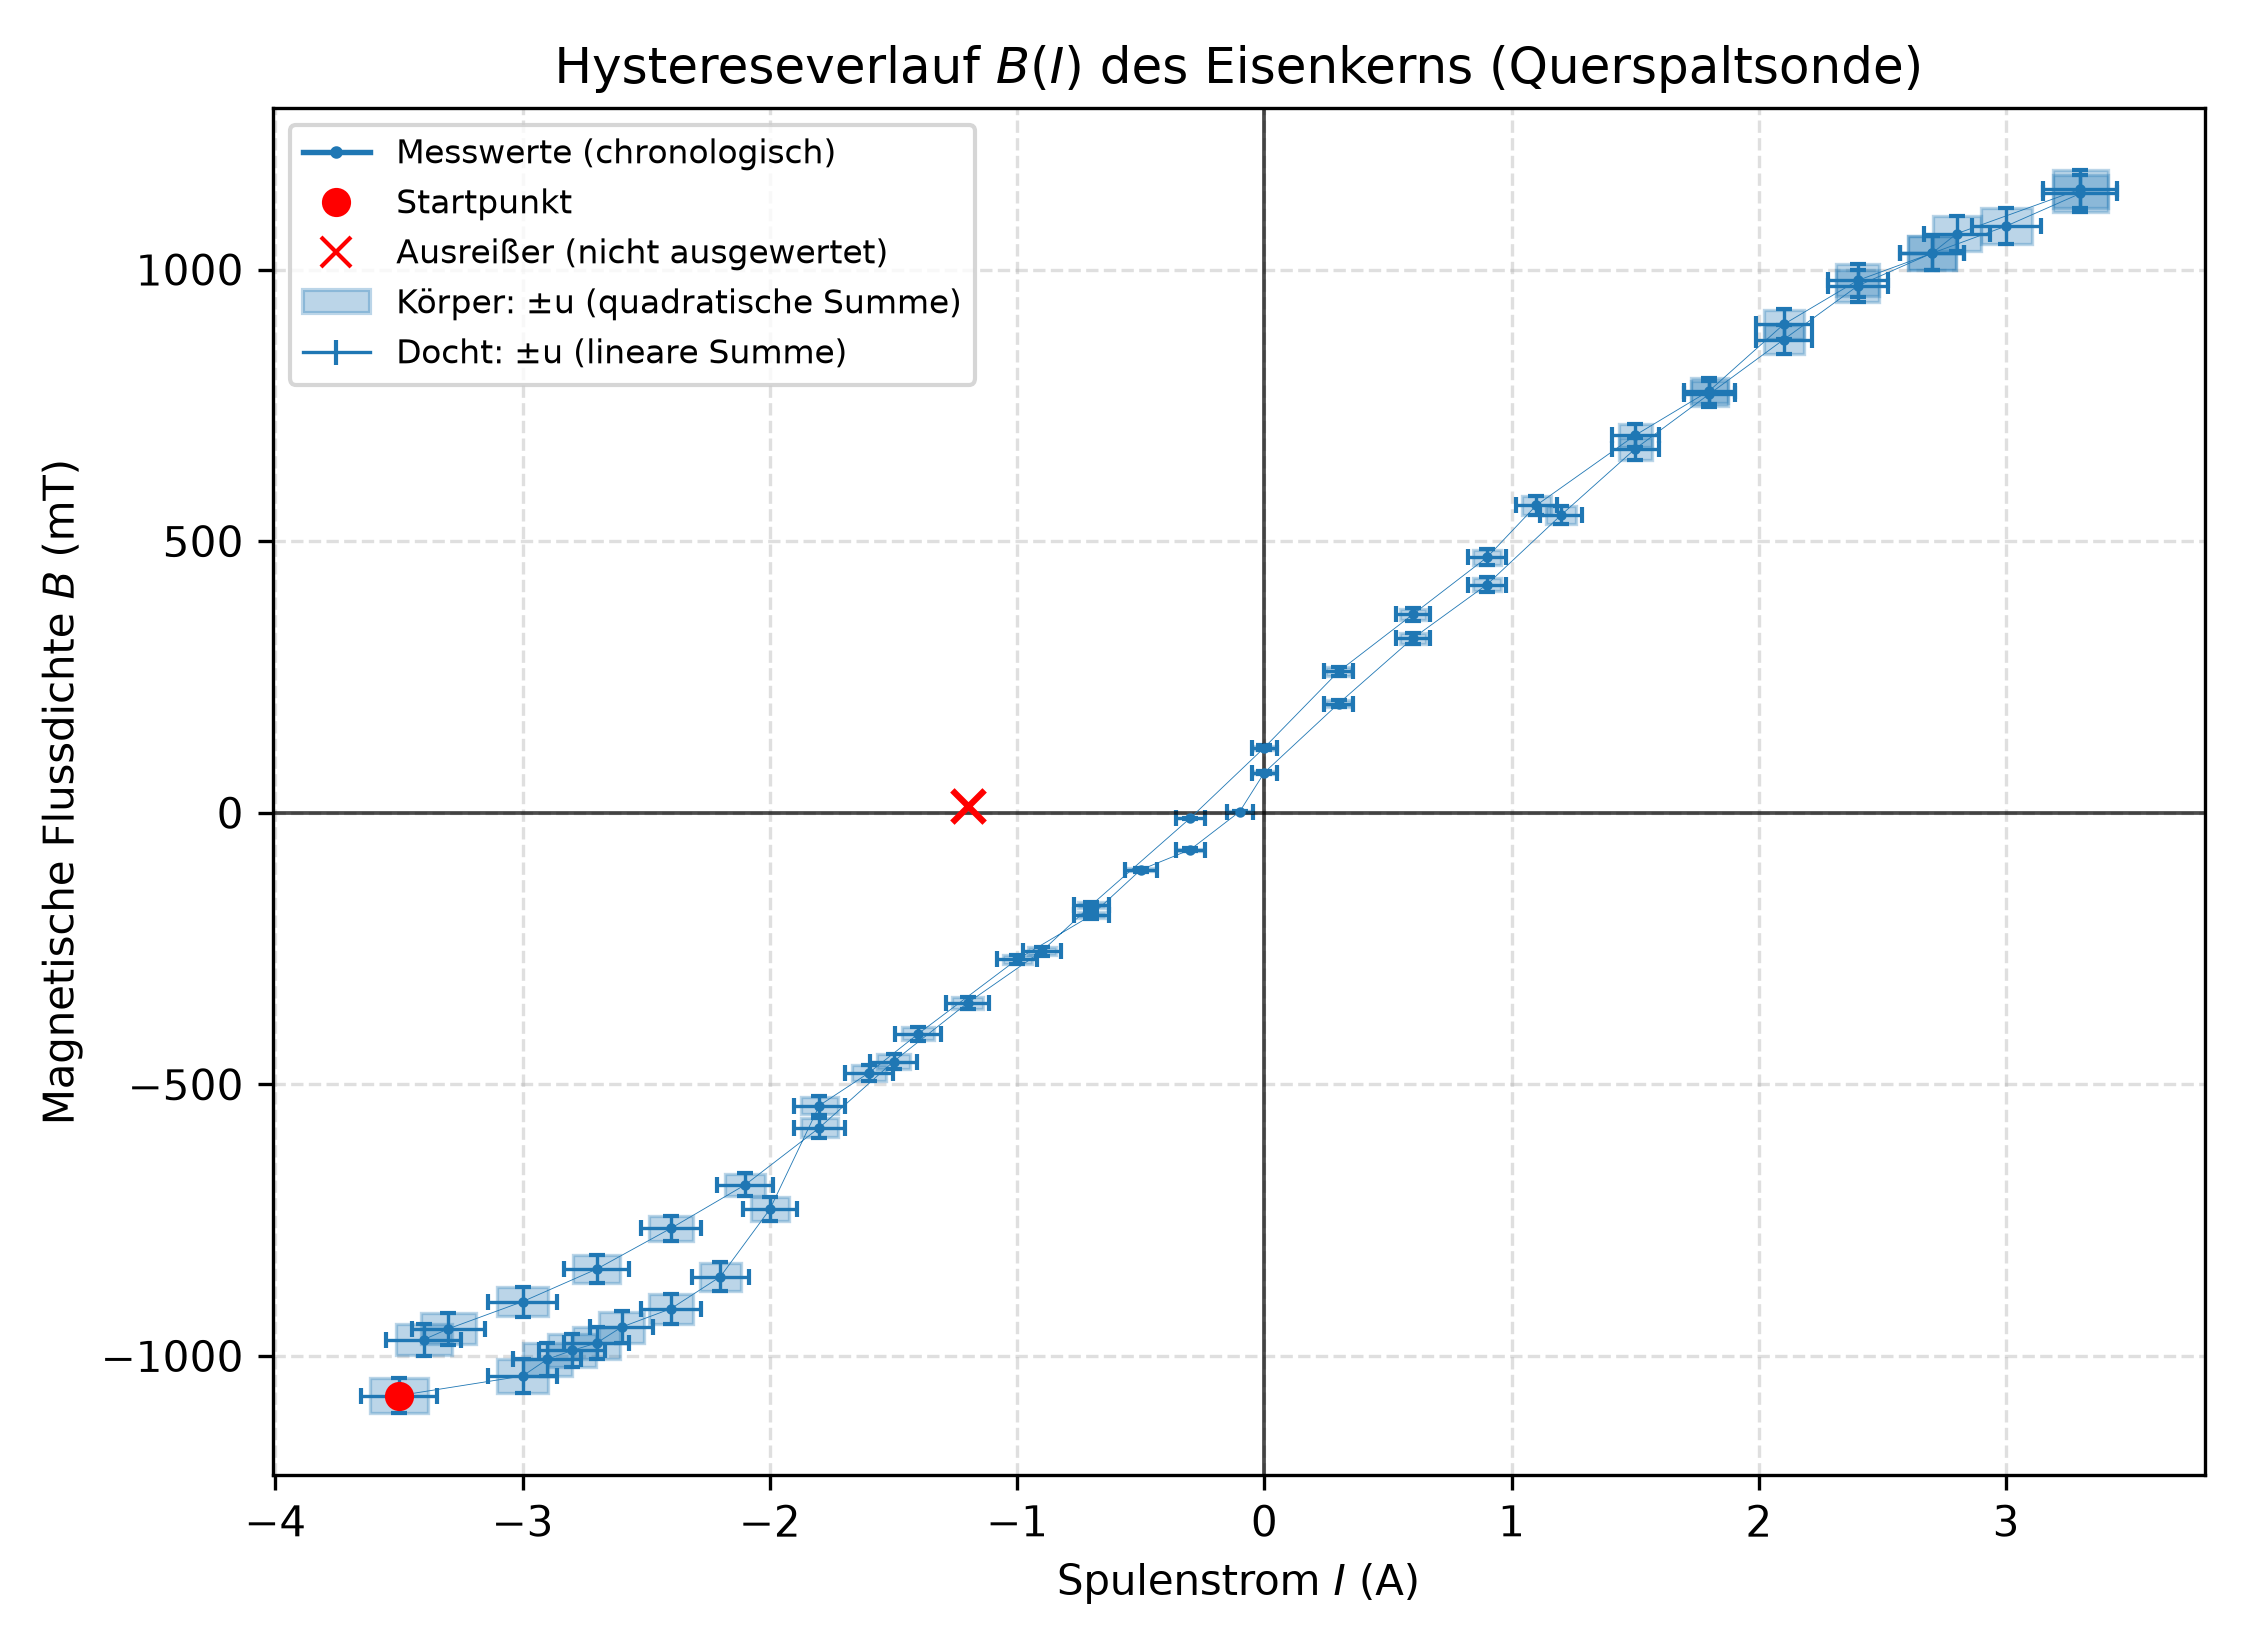
\includegraphics[width=0.85\textwidth]{hysterese_b_h.png}
  \caption{Hystereseverlauf: Flussdichte $B$ in Abhängigkeit vom Spulenstrom $I$
           (chronologische Reihenfolge, roter Punkt: Startpunkt bei etwa
           $-\SI{3.5}{\ampere}$). Die Polung des Stroms ist gegenüber der
           Anzeige umgekehrt, sodass $B$ mit $I$ ansteigt. Kerzen: Körper
           $=\pm u$ (quadratische Summe aus Ablesung, $\pm\SI{0.05}{\ampere}$
           bzw.\ $\pm\SI{0.5}{\milli\tesla}$, und \SI{3}{\percent}
           Geräteunsicherheit), Docht $=$ lineare Summe. Rotes Kreuz:
           vermuteter Aufzeichnungsfehler bei $I=-\SI{1.2}{\ampere}$ (nicht
           ausgewertet).}
  \label{fig:hysterese}
\end{figure}

\textbf{Beschreibung:} Die Kurve zeigt eine sehr schmale Hystereseschleife. Die
Achsenschnittpunkte beider Äste wurden aus den Messwerten linear interpoliert
und stehen in Tabelle~\ref{tab:hyst}.

\begin{table}[H]
  \centering
  \caption{Achsenschnittpunkte der beiden Äste (lineare Interpolation zwischen
           benachbarten Messpunkten, ohne den Ausreißer). Der Hinweg läuft mit
           steigendem, der Rückweg mit fallendem Strom.}
  \label{tab:hyst}
  \begin{tabular}{lcccc}
    \toprule
     & Hinweg & Rückweg & Mittelwert (Offset) & halbe Differenz \\
    \midrule
    $B$ bei $I=0$ & \SI{74}{\milli\tesla} & \SI{120}{\milli\tesla}
      & \SI{97}{\milli\tesla} & \SI{23}{\milli\tesla} \\
    $I$ bei $B=0$ & $-\SI{0.106}{\ampere}$ & $-\SI{0.277}{\ampere}$
      & $-\SI{0.191}{\ampere}$ & \SI{0.086}{\ampere} \\
    \bottomrule
  \end{tabular}
\end{table}

Bei einer um den Ursprung liegenden Schleife hätten die beiden Äste bei $I=0$
Flussdichten mit entgegengesetztem Vorzeichen, und die Nulldurchgänge lägen bei
Strömen mit entgegengesetztem Vorzeichen. Hier ist $B(I{=}0)$ auf beiden Ästen
positiv, und beide Nulldurchgänge liegen bei negativem Strom. Die Schleife ist
also gegenüber dem Ursprung verschoben, und zwar um etwa \SI{97}{\milli\tesla}
in $B$ bzw.\ \SI{0.19}{\ampere} in $I$. Beide Verschiebungen sind
größenordnungsmäßig verträglich: Der Quotient
$\SI{97}{\milli\tesla}/\SI{0.191}{\ampere}\approx\SI{0.5}{\tesla\per\ampere}$
liegt zwischen den mittleren Steigungen der beiden Äste zwischen $I=0$ und dem
jeweiligen Nulldurchgang ($\SI{74}{\milli\tesla}/\SI{0.106}{\ampere}\approx
\SI{0.7}{\tesla\per\ampere}$ bzw.\ $\SI{120}{\milli\tesla}/\SI{0.277}{\ampere}
\approx\SI{0.43}{\tesla\per\ampere}$). Es genügt daher ein Offset der
Flussdichte-Anzeige, vermutlich ein nicht abgeglichener oder gedrifteter
Nullpunkt der Querspaltsonde (ein Offset der Stromanzeige käme ebenfalls in
Frage). Unter der Annahme, dass der Offset die gesamte Schleife gleichmäßig
verschiebt, folgen $B_\mathrm{r}$ und $I_\mathrm{c}$ aus der halben Differenz
der Äste:
\begin{equation}
  B_\mathrm{r}\approx(23\pm2)\,\si{\milli\tesla},\qquad
  I_\mathrm{c}\approx(0.09\pm0.04)\,\si{\ampere}.
\end{equation}
Die Unsicherheiten ergeben sich aus einer groben Fehlerfortpflanzung der
Ablese- und Geräteunsicherheiten (Abschnitt~\ref{sec:unsicher}) und sind daher
nur eine Abschätzung. Gegenüber $B_\mathrm{max}\approx\SI{1.1}{\tesla}$ ist
$B_\mathrm{r}$ klein, der Aufbau wirkt magnetisch weich (eine schmale Schleife
bedeutet kleine Koerzitivfeldstärke).

Zu großen $|I|$ flacht die Kurve ab. Die Schleife schließt sich dort jedoch
nicht: Bei Strömen von \SIrange{2}{3}{\ampere} liegen die Äste etwa
\SIrange{80}{150}{\milli\tesla} auseinander. Start- und Endpunkt liegen bei
$-\SI{3.5}{\ampere}$ bzw.\ $-\SI{3.4}{\ampere}$ und unterscheiden sich in $B$ um
etwa \SI{100}{\milli\tesla} ($-\SI{1.07}{\tesla}$ gegenüber
$-\SI{0.97}{\tesla}$). Das spricht dafür, dass die Sättigung nicht erreicht
wurde.

\textbf{Anmerkungen zur Auswertung:}
\begin{itemize}
  \item \textbf{$B(I)$ statt $B(H)$:} Verlangt war ein $B(H)$-Diagramm.
        Mit der longitudinalen Sonde im Kern wurden sowohl in
        Abschnitt~\ref{sec:eisen} (Anzeige in der Bohrung bei null) als auch
        bei der Hysterese-Messung keine verwertbaren Werte erhalten. Die
        Ursache konnte nicht geklärt werden.
        Denkbar ist eine ungünstige Sondenposition in der Bohrung, belegt ist
        das nicht. Da damit keine Feldstärke $H$ vorliegt, wird $B$ über dem
        Spulenstrom aufgetragen. Eine Umrechnung mit $H\approx nI/l_\mathrm{m}$
        (vgl.\ fm.17) scheidet aus, da die mittlere Feldlinienlänge nicht
        bestimmt wurde. Außerdem ist $H_\mathrm{E}$ wegen des Querspalts nicht
        proportional zu $I$, sondern um den Beitrag des Spalts reduziert
        (Anleitung~\cite{anleitung}, Gl.~(fm.27):
        $H_\mathrm{E}=nI/l-M\,l_\mathrm{L}/l$). Die Schleife ist daher
        gegenüber $B(H_\mathrm{E})$ geschert, und $B(I{=}0)$ ist nicht die
        Remanenz des Materials. $B_\mathrm{r}$ und $I_\mathrm{c}$ sind
        Kenngrößen dieser Anordnung.
  \item \textbf{Vorzeichen:} Die Anzeige von $B$ hatte bezüglich der
        Stromanzeige das umgekehrte Vorzeichen (vermutlich wegen der
        Sondenorientierung bzw.\ der Polung). Für die Darstellung wurde das
        Vorzeichen des Stroms umgekehrt, sodass $B$ mit $I$ ansteigt. Da eine
        Hystereseschleife punktsymmetrisch ist, ändert das Form und Beträge
        nicht.
  \item \textbf{Ausreißer:} Der Messpunkt bei $I=-\SI{1.2}{\ampere}$ liegt mit
        $+\SI{12.0}{\milli\tesla}$ weit neben der Kurve (aus den Nachbarpunkten
        wären etwa $-\SI{340}{\milli\tesla}$ zu erwarten). Vermutlich handelt es
        sich um einen Fehler bei der handschriftlichen Aufzeichnung (schwer
        lesbare Ziffer oder Übertragungsfehler). Der Punkt wird als Ausreißer
        gewertet, im Plot gekennzeichnet und bei der Bestimmung von
        $B_\mathrm{r}$ und $I_\mathrm{c}$ nicht verwendet.
  \item \textbf{Sättigung:} Der Strom konnte nur bis etwa \SI{3.5}{\ampere}
        erhöht werden. Die Sättigung ist daher nicht eindeutig erreicht.
\end{itemize}

\clearpage

% ======================= 4 Diskussion / Fazit =======================
\section{Diskussion und Fazit}

\subsection{Messunsicherheiten}
\label{sec:unsicher}
Alle angegebenen Unsicherheiten sind Abschätzungen, keine Herstellerangaben.

\textbf{Spulenmessungen (Abschnitte~\ref{sec:luft} und~\ref{sec:eisen}):}
\begin{itemize}
  \item Geräte (Netzgerät, Hallsonde, Stromanzeige): \SI{3}{\percent} des Messwerts
  \item Ablesung: $\pm\SI{0.5}{\milli\tesla}$ (die Werte liegen ganzzahlig in
        \si{\milli\tesla} vor)
  \item Position: $\pm\SI{0.05}{\centi\meter}$, umgerechnet über die Steigung der
        Kurve, $u_{B,x}=|\mathrm{d}B/\mathrm{d}x|\cdot\SI{0.05}{\centi\meter}$.
        Der Beitrag beträgt in Experiment~1 höchstens etwa \SI{0.2}{\milli\tesla}.
        In Experiment~2 sind es an den steilsten Flanken in den dargestellten Kerzen
        (zentrale Differenz) bis etwa \SI{1.4}{\milli\tesla}, an der steilsten
        Einzelstufe ($-5{,}5$ bis $-\SI{5}{\centi\meter}$) etwa \SI{2}{\milli\tesla}.
\end{itemize}
Der Körper der Kerzen in den Abbildungen ist die quadratische Summe, der Docht
die lineare Summe (Worst Case).

\textbf{Hysterese (Abschnitt~\ref{sec:hyst}):} Die Flussdichte wurde auf
\SI{1}{\milli\tesla} genau abgelesen, der Strom auf \SI{0.1}{\ampere}. Als
Ablesefehler werden die halben Auflösungen angesetzt
($\pm\SI{0.5}{\milli\tesla}$ bzw.\ $\pm\SI{0.05}{\ampere}$), dazu jeweils
\SI{3}{\percent} Geräteunsicherheit. Quadratische Summe (Körper) und lineare
Summe (Docht) werden wie bei den Spulenmessungen dargestellt, hier in $B$ und $I$.
Bei großen Werten dominiert der relative Anteil (bei
$|B|\approx\SI{1}{\tesla}$ etwa \SI{30}{\milli\tesla}), die Ablesung ist
vernachlässigbar. Um $I=0$ beträgt die Unsicherheit der Flussdichte nur wenige
\si{\milli\tesla}. Die beobachteten Offsets (etwa \SI{97}{\milli\tesla} bzw.\
\SI{0.19}{\ampere}) liegen deutlich bzw.\ mehrfach darüber und sind daher
systematisch, nicht zufällig.

\textbf{Nicht erfasst} sind systematische Fehler. Dazu gehören die Verschiebung
des Nullpunkts der Position (etwa \SI{0.75}{\centi\meter} in
Abschnitt~\ref{sec:luft}), ein möglicher Offset der Sonden (in der Hysterese
etwa \SI{97}{\milli\tesla}), Verkippung oder Wackeln der Sonde und
Stromschwankungen, vor allem mit Eisenkern. Als weitere Einflüsse kommen
magnetische Störfelder aus der Umgebung in Frage. Die Länge des Eisenkerns und
die Eindringtiefe der longitudinalen Sonde wurden nicht gemessen, sodass die
Feldverläufe nicht mit der Kerngeometrie abgeglichen werden konnten.

Da der Versuch für alle Beteiligten die erste Laborerfahrung war, sind
zusätzliche Fehler wahrscheinlich: ungenaues Ablesen, Positionieren und
Ausrichten der Sonde sowie eine fehlerhafte Bestimmung und Umrechnung der
Spulenmitte, die die Verschiebung der Kurve um etwa \SI{0.75}{\centi\meter}
erklären dürfte. Diese Beiträge sind in den angegebenen Unsicherheiten nicht
enthalten. Die Messwerte wurden von Hand notiert und später übertragen. Dabei ist
vermutlich mindestens ein Aufzeichnungsfehler aufgetreten (Ausreißer in
Abschnitt~\ref{sec:hyst}). Bei einer Wiederholung sollten die Werte gemeinsam
laufend kontrolliert oder direkt digital erfasst werden.

\subsection{Fazit}
\begin{itemize}
  \item \textbf{Hallsonden:} Der Nullpunkt wurde am Erdmagnetfeld abgeglichen. Eine
        Aussage über die Empfindlichkeit der Sonden war damit nicht möglich.
  \item \textbf{Luftspule:} Der Feldverlauf ist glockenförmig und folgt
        qualitativ der Theorie der endlichen Zylinderspule. Das Maximum von
        \SI{16}{\milli\tesla} liegt \SI{7.5}{\percent} unter dem theoretischen
        Wert von \SI{17.3}{\milli\tesla}, nur schwach signifikant. Die Kurve ist
        um etwa \SI{0.75}{\centi\meter} verschoben, vermutlich durch eine falsch
        bestimmte Spulenmitte. Die Halbwertsbreite stimmt mit \SI{7.5}{\centi\meter}
        gegenüber \SI{8.0}{\centi\meter} annähernd mit der Theorie überein.
        Die Punktdipol-Näherung gilt nur im Fernfeld (ab etwa \SI{5}{\centi\meter}). Dort
        sind die Messwerte zu klein und zu grob aufgelöst, um den $|z|^{-3}$-Verlauf
        quantitativ zu prüfen.
  \item \textbf{Eisenkern:} In der Bohrung lag die Anzeige der longitudinalen
        Sonde über etwa \SI{7}{\centi\meter} bei null, eine Deutung war nicht
        möglich. An den Kernenden treten Maxima von etwa \SI{29}{\milli\tesla}
        und \SI{21}{\milli\tesla} auf, das größere am verjüngten Ende
        (Flusskonzentrator). Ein Wert für $\mu_\mathrm{r}$ ist aus diesen
        Messungen nicht bestimmbar: $B_\mathrm{E}$ liegt nur für den
        Hysterese-Aufbau vor, und in keinem Aufbau wurde ein auswertbares
        $H_\mathrm{E}$ erhalten.
  \item \textbf{Hysterese:} Statt des geforderten $B(H)$-Diagramms liegt $B(I)$
        vor, da keine auswertbare Feldstärke gemessen wurde. Die Messung zeigt
        eine sehr schmale Schleife mit $B_\mathrm{max}\approx\SI{1.1}{\tesla}$,
        $B_\mathrm{r}\approx\SI{23}{\milli\tesla}$ und
        $I_\mathrm{c}\approx\SI{0.09}{\ampere}$. Diese Kenngrößen gelten für die
        Anordnung mit Querspalt, nicht für das Material. Der Aufbau wirkt
        magnetisch weich. Die Schleife ist um etwa \SI{97}{\milli\tesla} bzw.\
        \SI{0.19}{\ampere} verschoben (vermutlich Offset der Querspaltsonde) und
        oben nicht geschlossen. Die Sättigung wurde nicht erreicht, da die
        Stromquelle nicht mehr lieferte. Ein Messpunkt ist vermutlich ein
        Aufzeichnungsfehler.
  \item \textbf{Verbesserungen:} Spulenmitte exakt bestimmen (Mitte der Wicklung)
        und die Position dokumentieren, Kernlänge und Sondenposition
        nachmessen, Nullpunkt der Querspaltsonde vor der Hysterese-Messung
        abgleichen, Mehrfachmessungen pro Punkt, eine zweite Stromquelle für
        Ströme bis \SI{5}{\ampere} und eine laufende bzw.\ digitale Erfassung der
        Messwerte.
\end{itemize}

\clearpage

\begin{thebibliography}{9}
  \bibitem{anleitung} Anleitung zum Anfängerpraktikum B, Versuch \glqq fm\grqq:
    Ferromagnetismus, 4.~Auflage 2019, Universität Regensburg.
\end{thebibliography}

\appendix
\section{Messwerte}
\begin{longtable}{rr@{\hspace{2cm}}rr}
\caption{Messwerte der Luftspule (Abschnitt~\ref{sec:luft}), unkorrigiert.}\label{tab:exp1}\\
\toprule
$x$ (cm) & $B$ (mT) & $x$ (cm) & $B$ (mT) \\
\midrule
\endfirsthead
\toprule
$x$ (cm) & $B$ (mT) & $x$ (cm) & $B$ (mT) \\
\midrule
\endhead
\bottomrule
\endfoot
-10,5 & 0 & 1 & 16 \\
-10 & 0 & 1,5 & 16 \\
-9 & 0 & 2 & 15 \\
-8 & 0 & 2,5 & 14 \\
-7 & 1 & 3 & 13 \\
-6,5 & 1 & 3,5 & 11 \\
-6 & 2 & 4 & 9 \\
-5,5 & 2 & 4,5 & 8 \\
-5 & 3 & 5 & 6 \\
-4,5 & 4 & 5,5 & 5 \\
-4 & 6 & 6 & 4 \\
-3,5 & 7 & 6,5 & 3 \\
-3 & 8 & 7 & 2 \\
-2,5 & 10 & 7,5 & 2 \\
-2 & 12 & 8 & 1 \\
-1,5 & 13 & 8,5 & 1 \\
-1 & 15 & 9 & 1 \\
-0,5 & 15 & 9,5 & 0 \\
0 & 16 & 10 & 0 \\
0,5 & 16 & 10,5 & 0 \\
\end{longtable}

\begin{longtable}{rr@{\hspace{2cm}}rr}
\caption{Messwerte der Spule mit Eisenkern (Abschnitt~\ref{sec:eisen}), unkorrigiert.}\label{tab:exp2}\\
\toprule
$x$ (cm) & $B$ (mT) & $x$ (cm) & $B$ (mT) \\
\midrule
\endfirsthead
\toprule
$x$ (cm) & $B$ (mT) & $x$ (cm) & $B$ (mT) \\
\midrule
\endhead
\bottomrule
\endfoot
-7 & 13 & 1 & 0 \\
-6,5 & 19 & 2 & 0 \\
-6 & 29 & 3 & 0 \\
-5,5 & 24 & 4 & 1 \\
-5 & 2 & 4,5 & 6 \\
-4,5 & 1 & 5 & 19 \\
-4 & 0 & 5,5 & 20 \\
-3 & 0 & 6 & 21 \\
-2 & 0 & 6,5 & 18 \\
-1 & 0 & 7 & 16 \\
0 & 0 &  &  \\
\end{longtable}

\begin{longtable}{rr@{\hspace{2cm}}rr}
\caption{Messwerte der Hysterese (Abschnitt~\ref{sec:hyst}) in chronologischer Reihenfolge, Rohwerte mit dem Stromvorzeichen der Anzeige (nicht umgepolt). $^{*}$\,Ausreißer (siehe Abschnitt~\ref{sec:hyst}).}\label{tab:exp3}\\
\toprule
$I$ (A) & $B$ (mT) & $I$ (A) & $B$ (mT) \\
\midrule
\endfirsthead
\toprule
$I$ (A) & $B$ (mT) & $I$ (A) & $B$ (mT) \\
\midrule
\endhead
\bottomrule
\endfoot
3,5 & -1073 & -2,7 & 1030 \\
3,0 & -1037 & -3,0 & 1080 \\
2,9 & -1006 & -3,3 & 1140 \\
2,8 & -990 & -3,3 & 1148 \\
2,7 & -976 & -2,8 & 1066 \\
2,6 & -947 & -2,7 & 1030 \\
2,4 & -913 & -2,4 & 980 \\
2,2 & -854 & -2,1 & 899 \\
2,0 & -730 & -1,8 & 777 \\
1,8 & -539 & -1,5 & 695 \\
1,6 & -479 & -1,1 & 566 \\
1,4 & -407 & -0,9 & 470 \\
1,2 & 12$^{*}$ & -0,6 & 365 \\
1,0 & -270 & -0,3 & 260 \\
0,7 & -189 & 0,0 & 120 \\
0,5 & -105 & 0,3 & -10 \\
0,3 & -68 & 0,7 & -170 \\
0,1 & 2 & 0,9 & -255 \\
0,0 & 74 & 1,2 & -350 \\
-0,3 & 201 & 1,5 & -458 \\
-0,6 & 321 & 1,8 & -580 \\
-0,9 & 420 & 2,1 & -685 \\
-1,2 & 548 & 2,4 & -765 \\
-1,5 & 670 & 2,7 & -840 \\
-1,8 & 771 & 3,0 & -900 \\
-2,1 & 871 & 3,3 & -950 \\
-2,4 & 970 & 3,4 & -970 \\
\end{longtable}


\end{document}
